\documentclass[a4paper,12pt]{article}

\usepackage{ifxetex}
\usepackage{amsmath,amssymb}
\ifxetex
	\usepackage{fontspec}
	\usepackage{polyglossia}
\else
	\usepackage{graphicx} % eps support
\fi
\usepackage[margin=20mm]{geometry}
\usepackage[colorlinks=true]{hyperref}
\urlstyle{same}
\usepackage{wrapfig}
\usepackage{caption}
\usepackage{subcaption}
\usepackage{authblk}
\usepackage{booktabs}
\usepackage{pstricks}
\usepackage{pstricks-add}
\usepackage[noabbrev,capitalize]{cleveref}

\newcommand\americium{${}^{241}$Am}
\newcommand\gadolinium{${}^{148}$Gd}
\newcommand\gainAm{$g_\text{Am}$}
\newcommand\gainGd{$g_\text{Gd}$}
\newcommand{\angstrom}{\mbox{\normalfont\AA}}


\title{The Study of the Silicon Detector Response for p-Carbon Polarization Measurements at RHIC}

\author[1]{D.~Kalinkin\thanks{dmitry.kalinkin@gmail.com}}
\author[2]{D.~Smirnov\thanks{d.s@plexoos.com}}

\affil[1]{Institute for Theoretical and Experimental Physics}
\affil[2]{Brookhaven National Laboratory}

\begin{document}

\maketitle

\begin{abstract}

At the Relativistic Heavy Ion Collider (RHIC) measurements of the proton beam
polarization are conducted by inserting an ultra thin carbon ribbon in the beam
and registering the scattered carbon ions with silicon detectors. The
polarization value reported by the proton-carbon polarimeters strongly depends
on the correct measurement of the energy deposited in the detectors by the
recoil products. In this note we present a study of the response of the silicon
detectors to $\alpha$-particles employed to calibrate the detectors.

\end{abstract}


\section{Motivation}

The RHIC polarimetry is based on the measurement of the recoil products from
elastic scattering of the proton beam on a fixed target in the Coulomb nuclear
interference (CNI) energy regime. In this study we focus on the four p-Carbon
polarimeters with ultra thin carbon targets which can be moved through
the beam. In the current setup the polarization of each proton beam can be
measured independently by two p-Carbon polarimeters installed in the ``yellow''
and ``blue'' accelerator rings.

During the 2013 run we observed significant changes in the gain in some of the
silicon detectors. This change of $\lesssim 20~\%$ is worrisome and may cause
significant systematic change in the reported polarization values due to a steep
slope in the $p$-Carbon analyzing power within the energy range of interest.


\section{Measurement and Results}

The detectors produced by the BNL instrumentation group have 12 one-millimeter
silicon strips operating under the nominal bias voltage of 110~V. The detector
gains are normally monitored by taking calibration runs when there is no beam in
the machine. Starting April 3, 2013 the calibration runs were taken
automatically at the end of every RHIC store immediately after the beam dump.
This approach allowed us to track the changes in detector properties at a more
precise level than before. Although we primarily focus on the Run~13 data we
also analyzed the data from $\alpha$-calibration runs in Run~12. The same analysis
procedure was performed on Run~12 data as well (see \cref{sec:appendix_run12}).
Because alpha runs weren't taken as frequently during Run~12, resulting plots for
it don't have as much statistics as the plots for Run~13.
The analysis of the data was performed with the {\tt cnipol} package~\cite{cnipol_code}.


\subsection{Energy calibration with $\alpha$-particles}

\begin{figure}[p]
\begin{subfigure}[t]{0.49\textwidth}
\setlength{\unitlength}{0.075\textwidth}
\psset{unit=\unitlength}

\begin{pspicture}(0,0)(12,11) % for debugging add [showgrid=true]

% yaxe
\psStartPoint(2.4,1)\psVector(0,10)
\rput[r](2,10){ADC}

% xaxe
\psStartPoint(2,1.4)\psVector(10,0)
\rput[t](11,1){E}

% adc americium tick
\psline(2.2,8)(2.6,8)
\rput[r](2,8){$\mu_\text{Am}$}

% adc gadolinium tick
\psline(2.2,5)(2.6,5)
\rput[r](2,5){$\mu_\text{Gd}$}

\psline(4,1)(10,9)

\psline(4.3,1.2)(4.3,1.6)
\rput[lt](4.3,1){$E_\text{DL}$}

\psline(7,1.2)(7,1.6)
\rput[t](7,1){$E_\text{Gd}$}

\psline(9.2,1.2)(9.2,1.6)
\rput[t](9.2,1){$E_\text{Am}$}

\end{pspicture}
 \caption{Missing energy $E_\text{DL}$ can be
defined in the approximation of energy deposition independent of the particle
energy.}
\label{fig:calib_curve_naive}
\end{subfigure}
\hfill
\begin{subfigure}[t]{0.49\textwidth}
\setlength{\unitlength}{0.075\textwidth}
\psset{unit=\unitlength}

\begin{pspicture}(0,0)(12,11) % for debugging add [showgrid=true]

% yaxe
\psStartPoint(2.4,1)\psVector(0,10)
\rput[r](2,10){$x_\text{registered}$}

% xaxe
\psStartPoint(2,1.4)\psVector(10,0)
\rput[t](11,1){$x_\text{total}$}

% adc americium tick
\psline(2.2,8)(2.6,8)
\rput[r](2,8){$\frac{\mu_\text{Am}}{g \cdot \lambda_\text{Am}}$}

% adc gadolinium tick
\psline(2.2,5)(2.6,5)
\rput[r](2,5){$\frac{\mu_\text{Gd}}{g \cdot \lambda_\text{Gd}}$}

\psline(4,1)(10,9)

\psline(4.3,1.2)(4.3,1.6)
\rput[lt](4.3,1){$x_\text{DL}$}

\psline(7,1.2)(7,1.6)
\rput[t](7,1){$\frac{E_\text{Gd}}{\lambda_\text{Gd}}$}

\psline(9.2,1.2)(9.2,1.6)
\rput[t](9.2,1){$\frac{E_\text{Am}}{\lambda_\text{Am}}$}

\end{pspicture}

\caption{Dead layer size $x_\text{DL}$ is a difference between the distance
that particle traveled trough the matter $x_\text{total}$ and a distance on
which the deposited energy was being registered by the detector
$x_\text{registered}$.  Gain relation $g=g_\text{Am}=g_\text{Gd}$ is assumed.
The linear regression gives us \cref{eq:x_dl}.  Note that the result does not
depend on the value of gain $g$.}
\label{fig:calib_curve_smart}
\end{subfigure}
\caption{Definition of $E_\text{DL}$ and $x_\text{DL}$ in terms of linear regression
over two points corresponding to two alpha sources.}
\label{fig:calib_curves}
\end{figure}

In order to perform a polarization measurement we need to measure the energy of
the slow carbon ions coming from the fixed target. The calorimetry is done by
utilizing the silicon strip detectors introduced above.  We observe that
signals coming from the detectors have the same shape.  Thus each signal can be
parametrized with only one parameter.  We use that parameter to reconstruct the
energy of the recoil particle.  As of Run~2013 the data from pCarbon
polarimeters comes in a form of a two quantities: the maximum amplitude and the
total charge (i.e. integral). On the contrary, H-Jet data comes in full
waveforms. In agreement with signals affinity, we observe a very good correlation
between the maximum amplitude and the integral of the collected charge. Our
choice of the former is only set by convention.
For the energy calibration purposes we use low intensity \americium{} and \gadolinium{} radioactive
sources emitting $\alpha$-particles with fixed energies of $E_{\text{Am}} =
5.486~\text{MeV}$ and $E_{\text{Gd}} = 3.183~\text{MeV}$\cite{rytz} respectively. The
sources are put inside the vacuum of the beam pipe in the direct acceptance of the detectors. In
2012 and 2013 two polarimeters, Y1D and B1U (see \cref{fig:polarim_placement}), were supplied with \americium{}
sources only, while the other two, Y2U and B2D, had, in addition, \gadolinium{}
sources installed inside the polarimeter chambers. Prior to 2012 only the
americium sources were available for calibration.

The energy of the $\alpha$-particles is few times higher than that of the
carbon ions reaching the detectors. We reduce the output signal by means of
attenuators by a factor of five to bring it back to the range where the
amplitude can be digitized by the readout electronics. In the absence of the
beam we observe clean peaks from the radioactive sources as shown in
\cref{fig:atten_distrib_nominal}. The peaks positions are determined using a
gaussian function fit.

The current offline analysis is only based on a calibration with the \americium{} source.
The nominal detector gain \gainAm{} is
defined as a ratio of the peak position, $\mu_{\text{Am}}$, to the
$E_{\text{Am}}$ energy. This definition completely ignores possible energy
losses before the sensitive detector region. This limitation can be overcome
to some extent by using a second $\alpha$-source. With two sources the slope of
a linear calibration curve effectively takes into account the unresponsive
region of the detector as illustrated with a sketch in
\cref{fig:calib_curves}. This region is referred to as the {\it dead
layer}, and we discuss it in the next section.

\Cref{fig:gainAm} shows how the americium gain \gainAm{} developed in time for all
four p-Carbon polarimeters. From this we conclude that overall gain was
stable on a monthly scale with only few detectors showing up to 20\%
instabilities in the gain. We also confirm an overall stability by looking at
the ratio of the gain estimate for the polarimeters with an additional
\gadolinium{} source. These quantities as a function of time are shown on
\cref{fig:gain_relations}.


\newcommand\amgainlabel{Time dependence of the detector gain $g_\text{Am}$ as
measured with $\alpha$-particles emitted by the \americium{} source. Colors
represent individual detectors.}

\begin{figure}
\begin{center}
\setlength{\unitlength}{0.035\textwidth}
\psset{unit=\unitlength}

\begin{pspicture}(0,0)(10,10) % for debugging add [showgrid=true]

\psline(1,5)(9,5)
\rput[r](1,5){Det2}
\rput[l](9,5){Det5}

%  2.17 = 5-cos(45)*4
%  7.82 = 5+cos(45)*4
\psline(2.17,2.17)(7.82,7.82)
\rput[r](2.17,2.17){Det3}
\rput[l](7.82,7.82){Det6}

\psline(2.17,7.82)(7.82,2.17)
\rput[r](2.17,7.82){Det1}
\rput[l](7.82,2.17){Det4}

\end{pspicture}

\end{center}
\caption{Schematic view of the detector alignment in the plane perpendicular to
the beam. Carbon strip target is aligned vertically, detectors are aligned at
angles $45^\circ$, $90^\circ$, $135^\circ$ to it. The beam points into the
figure perpendiculary.}
\end{figure}

\begin{figure}
\begin{center}
\setlength{\unitlength}{0.035\textwidth}
\psset{unit=\unitlength}

\begin{pspicture}(0,0)(20,5) % for debugging add [showgrid=true]

\psset{linewidth=2pt,arrowscale=2}

\newcommand\bluering{
\psarc			(10,-15){18}{60}{90}
\psarc[arrows=<-]	(10,-15){18}{72}{82}
\psarc			(10,-15){19}{90}{120}
\psarc[arrows=<-]	(10,-15){19}{102}{112}
}

\psset{linecolor=cyan,origin={-0.05,-0.05}}
\bluering
\psset{origin={0,0}}

\psset{linecolor=blue}
\bluering

\newcommand\yellowring{
\psarc			(10,-15){19}{60}{90}
\psarc[arrows=->]	(10,-15){19}{75}{76}
\psarc			(10,-15){18}{90}{120}
\psarc[arrows=->]	(10,-15){18}{105}{106}
}

\psset{linecolor=orange,origin={-0.05,-0.05}}
\yellowring
\psset{origin={0,0}}

\psset{linecolor=yellow}
\yellowring

\psset{linecolor=magenta,fillcolor=magenta}
\pscircle*(10,3.5){0.85}
\pscircle*(12.31,3.86){0.3}
\pscircle*(13.3,3.71){0.3}
\pscircle*(12.31,2.86){0.3}
\pscircle*(13.3,2.72){0.3}

\rput[c](10,4.8){HJet}
\rput[c](11.9,4.5){Y1D}
\rput[c](13.5,4.3){Y2U}
\rput[c](11.9,2.2){B1U}
\rput[c](13.5,2.0){B2D}

\end{pspicture}

\end{center}
\caption{Schematic view of polarimeters placement around IP12.}
\label{fig:polarim_placement}
\end{figure}

\begin{figure}
%
\begin{subfigure}[t]{0.49\textwidth}
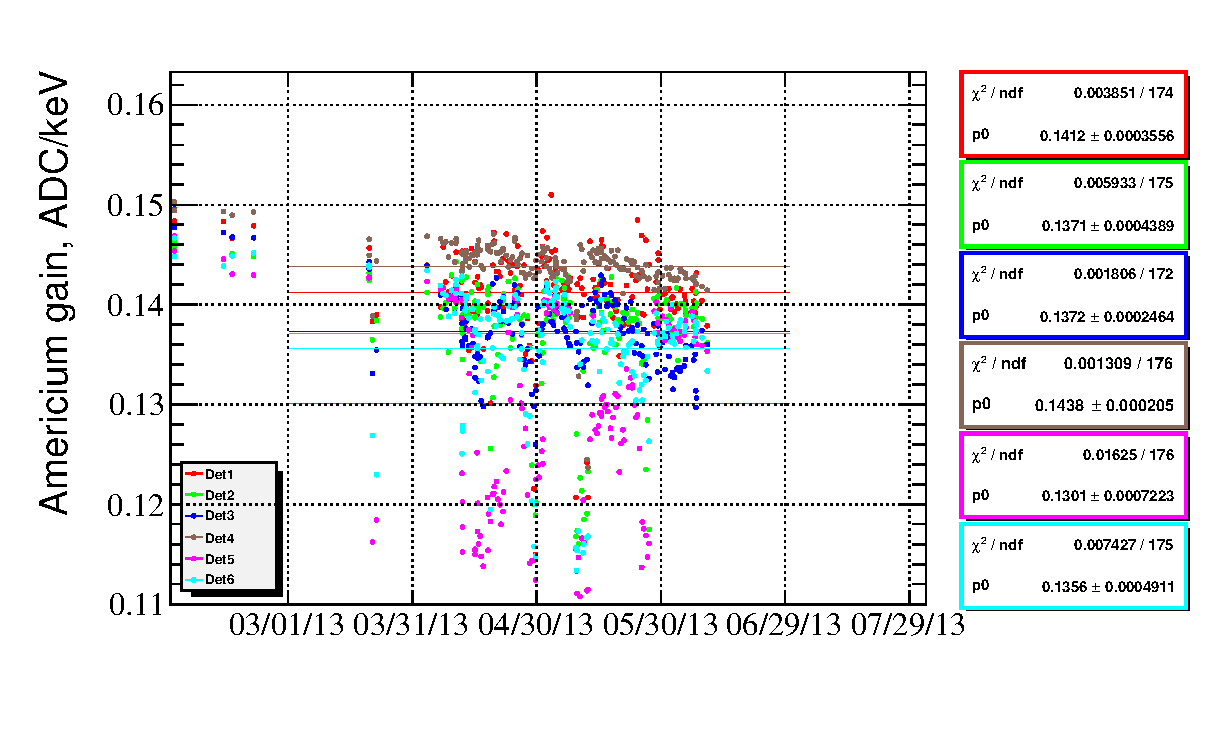
\includegraphics[width=\textwidth]{gfx/run13_alpha_study_novoltagevariation/B1U/c_chAmGain_by_day_B1U.eps}
\caption{B1U}
\end{subfigure}
%
\hfill
%
\begin{subfigure}[t]{0.49\textwidth}
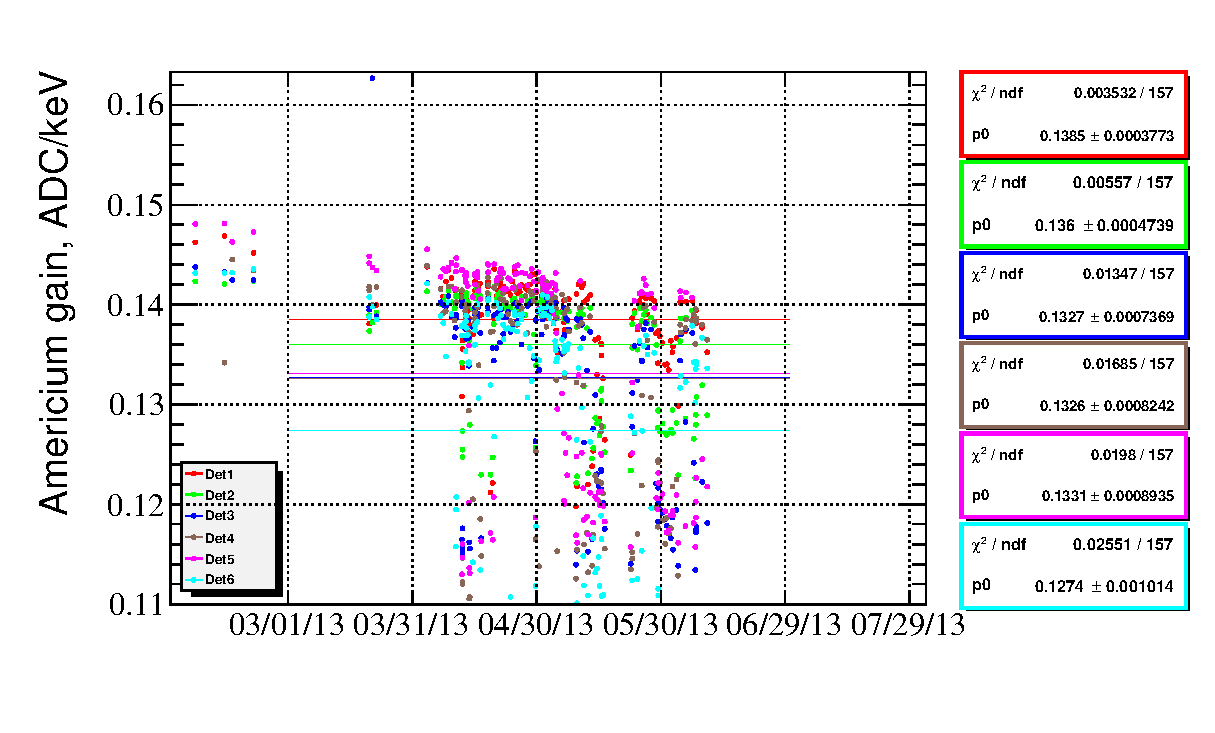
\includegraphics[width=\textwidth]{gfx/run13_alpha_study_novoltagevariation/Y1D/c_chAmGain_by_day_Y1D.eps}
\caption{Y1D}
\end{subfigure}
%
\begin{subfigure}[t]{0.49\textwidth}
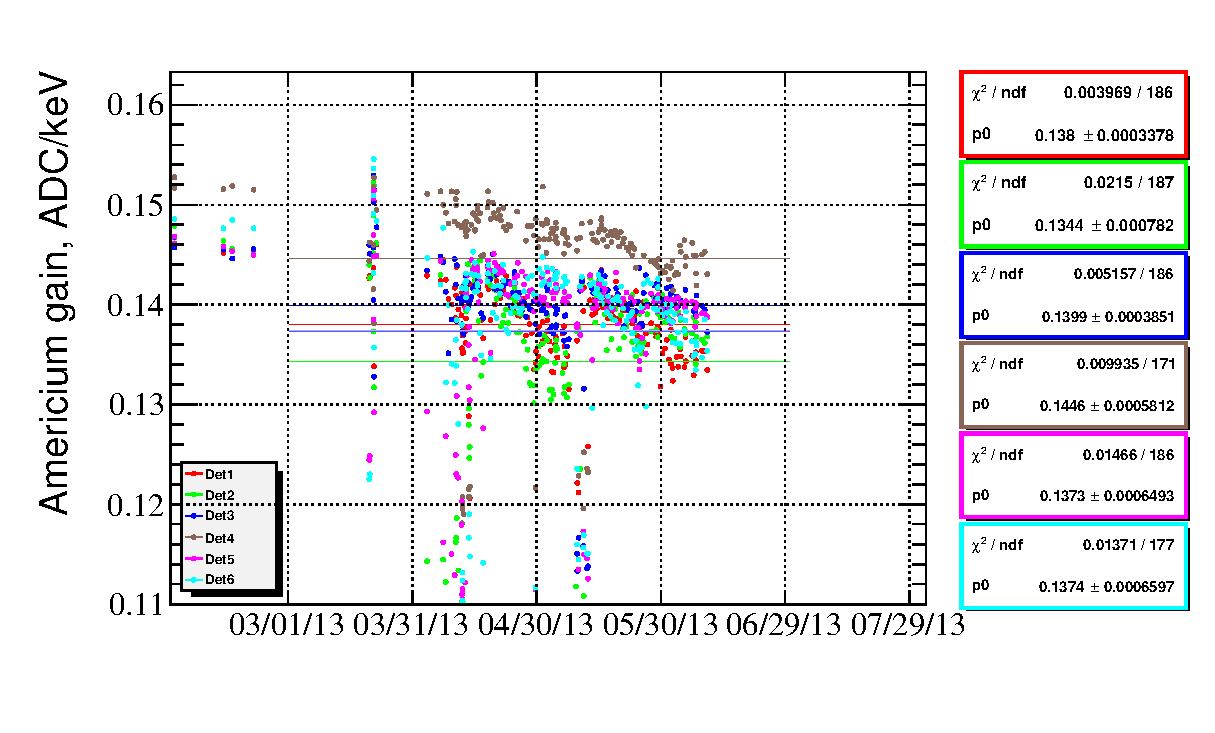
\includegraphics[width=\textwidth]{gfx/run13_alpha_study_novoltagevariation/B2D/c_chAmGain_by_day_B2D.eps}
\caption{B2D}
\end{subfigure}
%
\hfill
%
\begin{subfigure}[t]{0.49\textwidth}
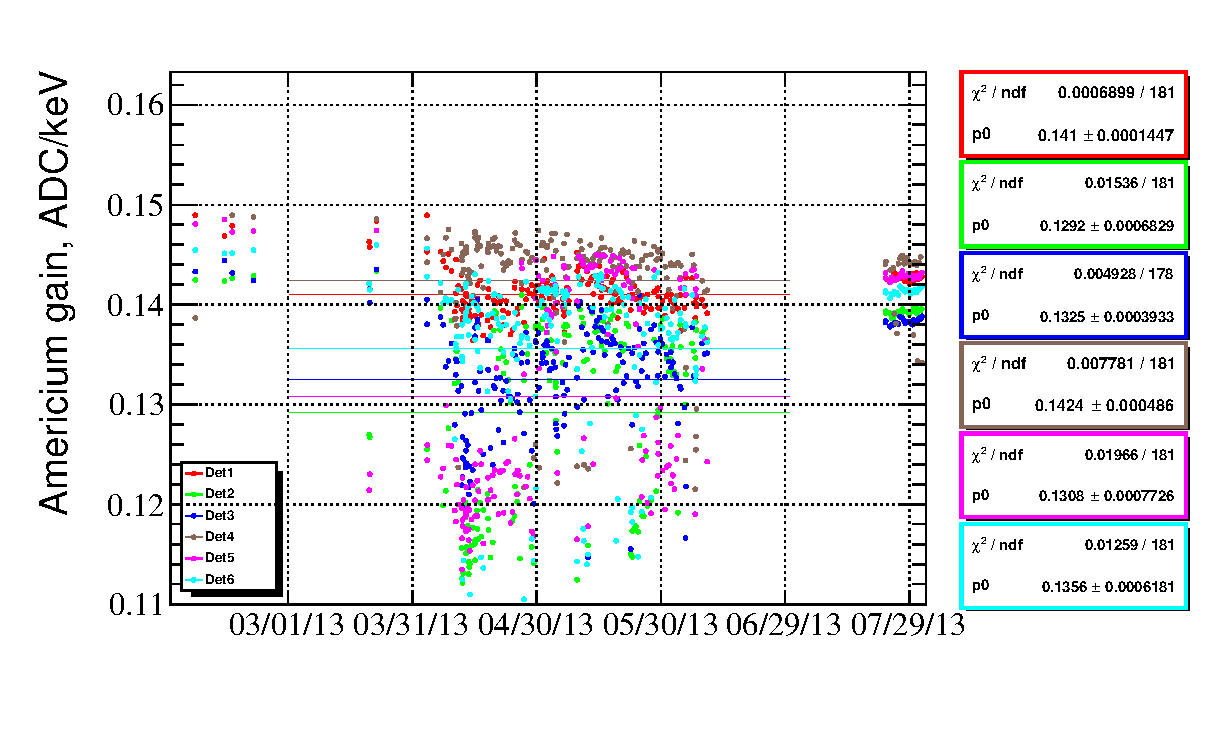
\includegraphics[width=\textwidth]{gfx/run13_alpha_study_novoltagevariation/Y2U/c_chAmGain_by_day_Y2U.eps}
\caption{Y2U}
\end{subfigure}
%
\caption{\amgainlabel{}}
\label{fig:gainAm}
\end{figure}


\newcommand\gainrealationslabel{Comparison of the effective detector gains
calculated with either one or both $\alpha$-sources for the polarimeters
equipped with two alpha sources. Colors represent individual detectors.}
\begin{figure}
%
\begin{subfigure}[t]{0.49\textwidth}
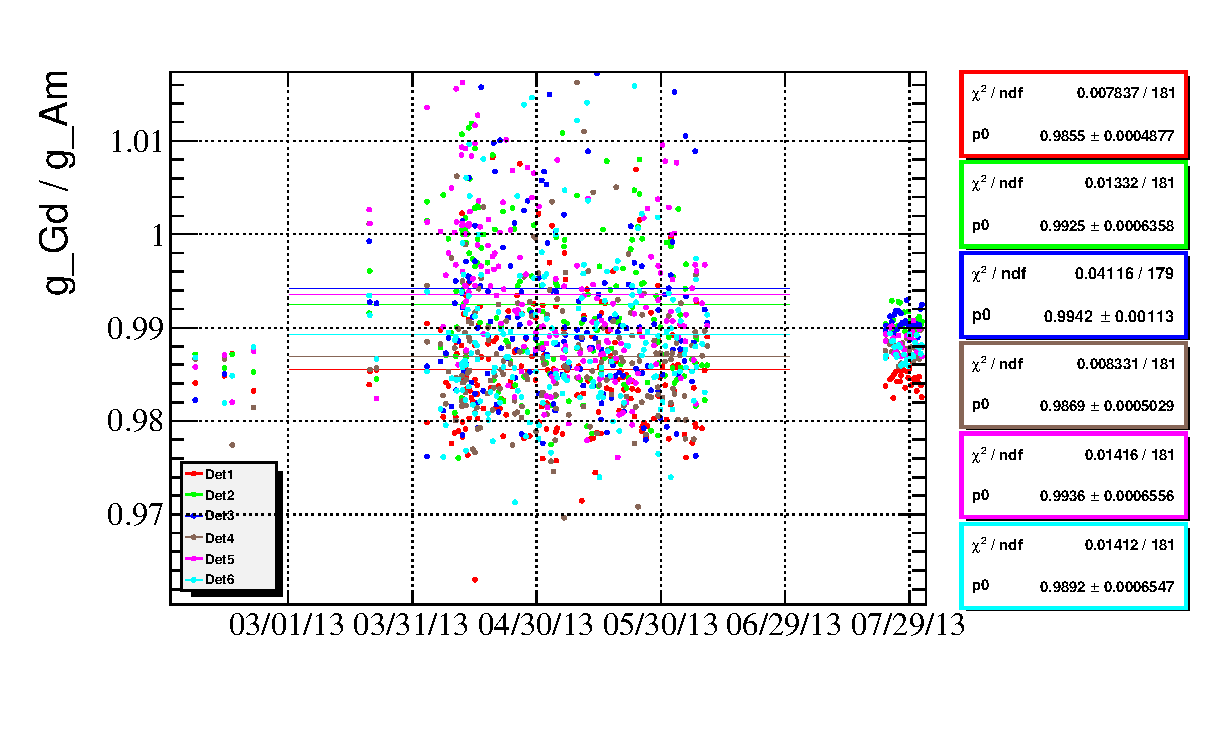
\includegraphics[width=\textwidth]{gfx/run13_alpha_study_novoltagevariation/Y2U/c_chGdGain_over_AmGain_by_day_Y2U.eps}
\caption{Time dependence of the ratio of the gains, $g_\text{Gd}/g_\text{Am}$,
independently measured with \gadolinium{} and \americium{} sources for
\textbf{Y2U} polarimeter.}
\end{subfigure}
%
\hfill
%
\begin{subfigure}[t]{0.49\textwidth}
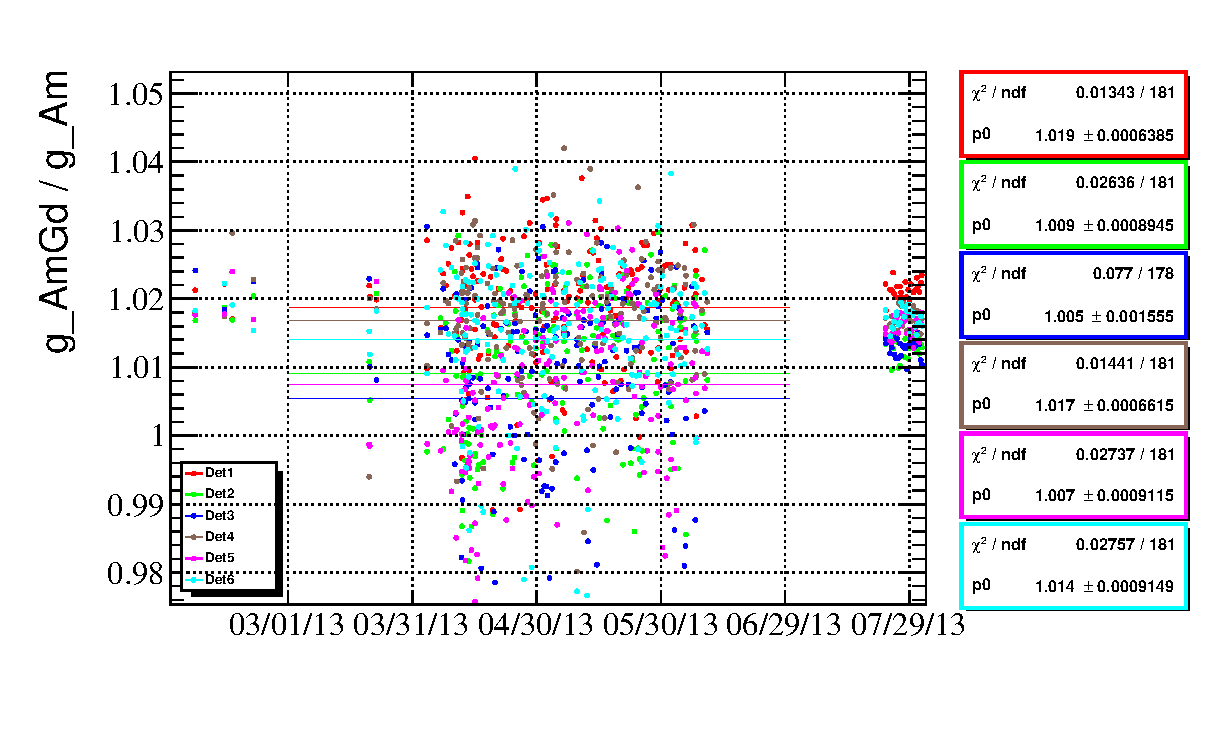
\includegraphics[width=\textwidth]{gfx/run13_alpha_study_novoltagevariation/Y2U/c_chAmGdGain_over_AmGain_by_day_Y2U.eps}
\caption{Time dependence of the ratio of the gain measured with both \americium{} and
\gadolinium{} sources to the nominal gain measured with only the \americium{}
source for \textbf{Y2U} polarimeter.}
\end{subfigure}
%
\begin{subfigure}[t]{0.49\textwidth}
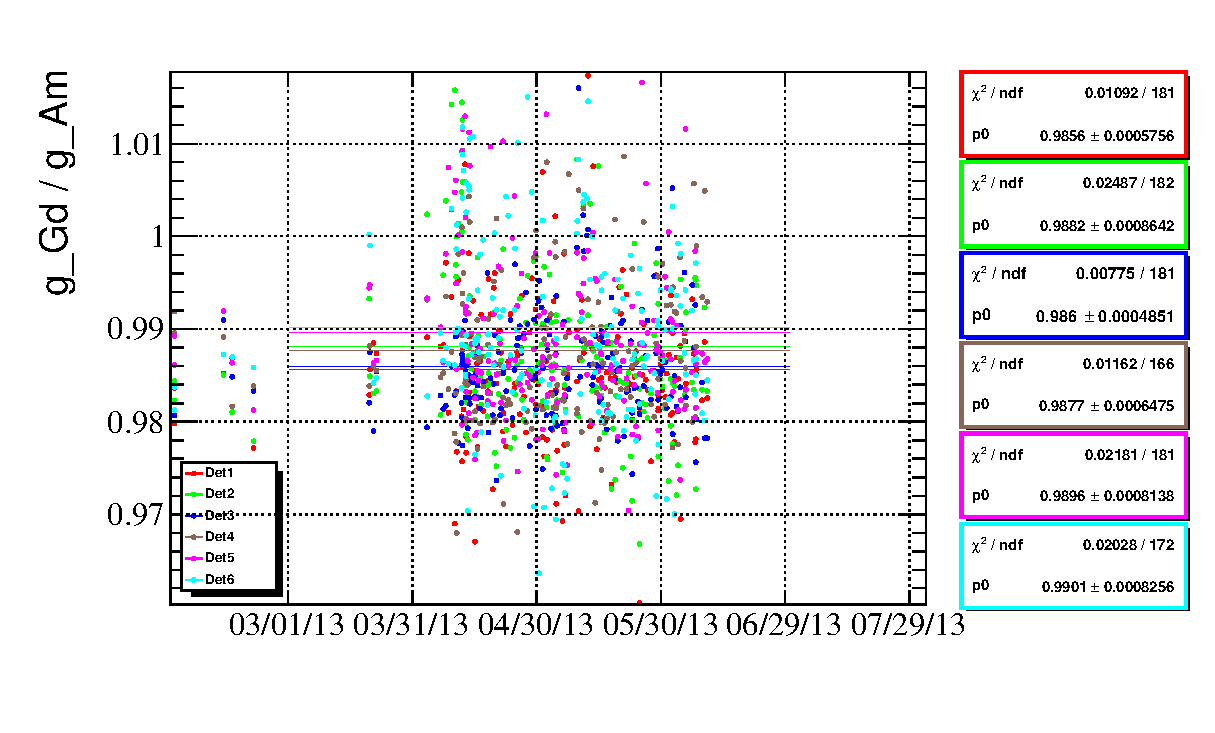
\includegraphics[width=\textwidth]{gfx/run13_alpha_study_novoltagevariation/B2D/c_chGdGain_over_AmGain_by_day_B2D.eps}
\caption{Time dependence of the ratio of the gains, $g_\text{Gd}/g_\text{Am}$,
independently measured with \gadolinium{} and \americium{} sources for
\textbf{B2D} polarimeter.}
\end{subfigure}
%
\hfill
%
\begin{subfigure}[t]{0.49\textwidth}
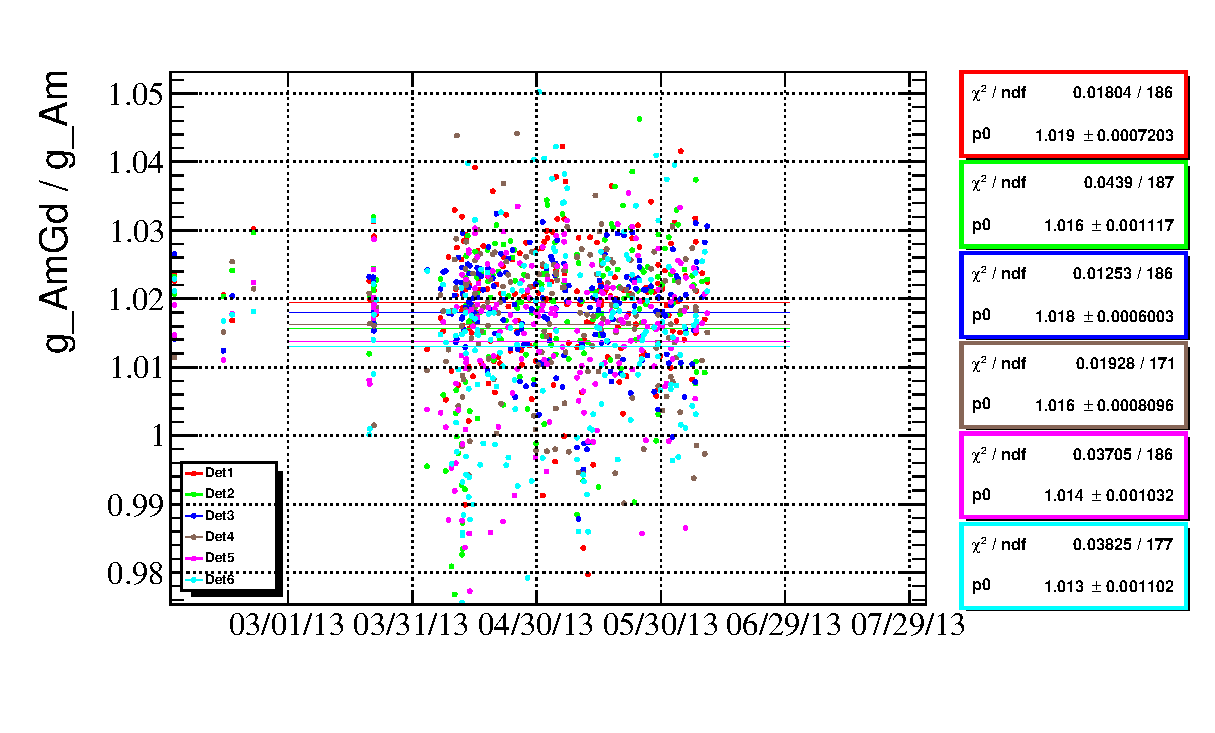
\includegraphics[width=\textwidth]{gfx/run13_alpha_study_novoltagevariation/B2D/c_chAmGdGain_over_AmGain_by_day_B2D.eps}
\caption{Time dependence of the ratio of the gain measured with both \americium{} and
\gadolinium{} sources to the nominal gain measured with only the \americium{}
source for \textbf{B2D} polarimeter.}
\end{subfigure}
\caption{\gainrealationslabel{}}
\label{fig:gain_relations}
\end{figure}


\subsection{Effective dead layer}

In our current model of the silicon detector the incident particles are assumed
to pass through a region where the detector has zero response as a calorimeter,
i.e. the dead layer. Adding a gadolinium alpha source to the setup allows us to
put one more calibration point on our calibration curve (see
\cref{fig:calib_curves}). With the points corresponding to the americium
and gadolinium sources we can estimate the thickness of this layer.

The energy where the linear fit intersects the horizontal axis gives us an
estimate for the initial energy of incident $\alpha$-particles which would
deposit all of their energy in the dead layer. While this quantity by itself
can be used to monitor the stability of the effective dead layer over time, we also
present the result in $\mu g/cm^2$. For the latter, we assume that the detector
response to the both incident energies is the same, and we write:

\begin{equation}
\frac{\mu_{Am}}{E_{Am} - E^\text{DL}_{Am}} = \frac{\mu_{Gd}}{E_{Gd} - E^\text{DL}_{Gd}},
\label{eq:gain_equality}
\end{equation}

\noindent where $\mu_\text{Am}$ and $\mu_\text{Gd}$ are the mean values of the
alpha peaks measured in ADC units, $E_\text{Am}$ and $E_\text{Gd}$ are the
incident energies of $\alpha$-particles, and $E^\text{DL}_{Am}$ and
$E^\text{DL}_{Gd}$ are the energy losses in the dead layer for the respective
alpha sources.

\begin{figure}
\begin{subfigure}[b]{0.5\textwidth}
\includegraphics[width=\textwidth]{astar_plots/csda_range.eps}
\caption{CSDA versus alpha particle energy}\label{subfig:csda_range}
\end{subfigure}
\begin{subfigure}[b]{0.5\textwidth}
\includegraphics[width=\textwidth]{astar_plots/stopping_power.eps}
\caption{Stopping power versus penetration depth}\label{subfig:stopping_power}
\end{subfigure}
\caption{}\label{fig:astar_plots}
\end{figure}

The rate at which $\alpha$-particles loose their energy in the detector changes
with the penetration depth. The value of stopping power can be easily derived
from the \emph{CSDA range}\footnotemark values available at the
ASTAR Database\cite{astar_database}.

\footnotetext{The \emph{CSDA range} is a very close approximation to the
average path length traveled by a charged particle as it slows down to rest,
calculated in the continuous-slowing-down approximation. In this approximation,
the rate of energy loss at every point along the track is assumed to be equal
to the total stopping power. Energy-loss fluctuations are neglected. The CSDA
range is obtained by integrating the reciprocal of the total stopping power
with respect to energy. -- ASTAR Appendix: Significance of Calculated
Quantities}

The original CSDA range data for $\alpha$-particles is displayed in
\cref{subfig:csda_range}. If we take CSDA range value for the
$E=E_{\text{Am}}$ and $E=E_{\text{Gd}}$ we will get maximal penetration depths
$z^0_{\text{Am}}$, $z^0_{\text{Gd}}$.  Penetration depth is then calculated as
$z_i = z^0_i - \text{CSDA\:range}$.  Stopping power $-\frac{dE}{dz_i}$ can be
then derived from $E$ vs $z_i$ points using simple numerical differentiation formula
$\frac{df}{dx} = (f_{i+1} - f_i)/(x_{i+1} - x_i)$. The resulting plot for
stopping power versus penetration depth can be seen in \cref{subfig:stopping_power}.
This plot is consistent with the other plot\cite{schmidke_edep} of the same dependency, derived from
the data from the same ASTAR Database, but using a different method.

As the dead layer is relatively thin (less than $1\text{ }\mu\text{m}$)
$\alpha$-particles do not loose a significant fraction of their initial energy
and the stopping power is approximately constant over this range. With a linear
approximation for the total losses we have:

\begin{equation}
E^\text{DL}_\text{Am} \simeq x_\text{DL} \lambda_\text{Am} \qquad
E^\text{DL}_\text{Gd} \simeq x_\text{DL} \lambda_\text{Gd}
\label{eq:linear_loss}
\end{equation}

\noindent
with values for the stopping power $\lambda_\text{Am} = 140\text{ keV/}\mu m$
and $\lambda_\text{Gd} = 190\text{ keV/}\mu m$ taken from the plot on
\cref{subfig:stopping_power} at $z=0$. Combining \cref{eq:gain_equality,eq:linear_loss}
we obtain the following formula for the size of the effective dead layer:

\begin{equation}
x_{DL} = \frac{\mu_{Gd} E_{Am} - \mu_{Am} E_{Gd}}{\mu_{Gd}\lambda_{Am} - \mu_{Am}\lambda_{Gd}}
\label{eq:x_dl}
\end{equation}

This formula could be also realized as a linear regression fit of the plot at
\cref{fig:calib_curve_smart}.

The thickness of the dead layer thus extracted from the all available
calibration runs in Run~13 are shown in \cref{fig:x_dl}. The average size
of the effective dead layer is estimated to be within 80 to 100 $\mu g/cm^2$.

\newcommand\edllabellabel{$E_{DL}$ (see \cref{fig:calib_curve_naive}) is the missing
energy value extracted from linear fit of the americium and gadolinium points.}
\begin{figure}
\begin{subfigure}[b]{0.5\textwidth}
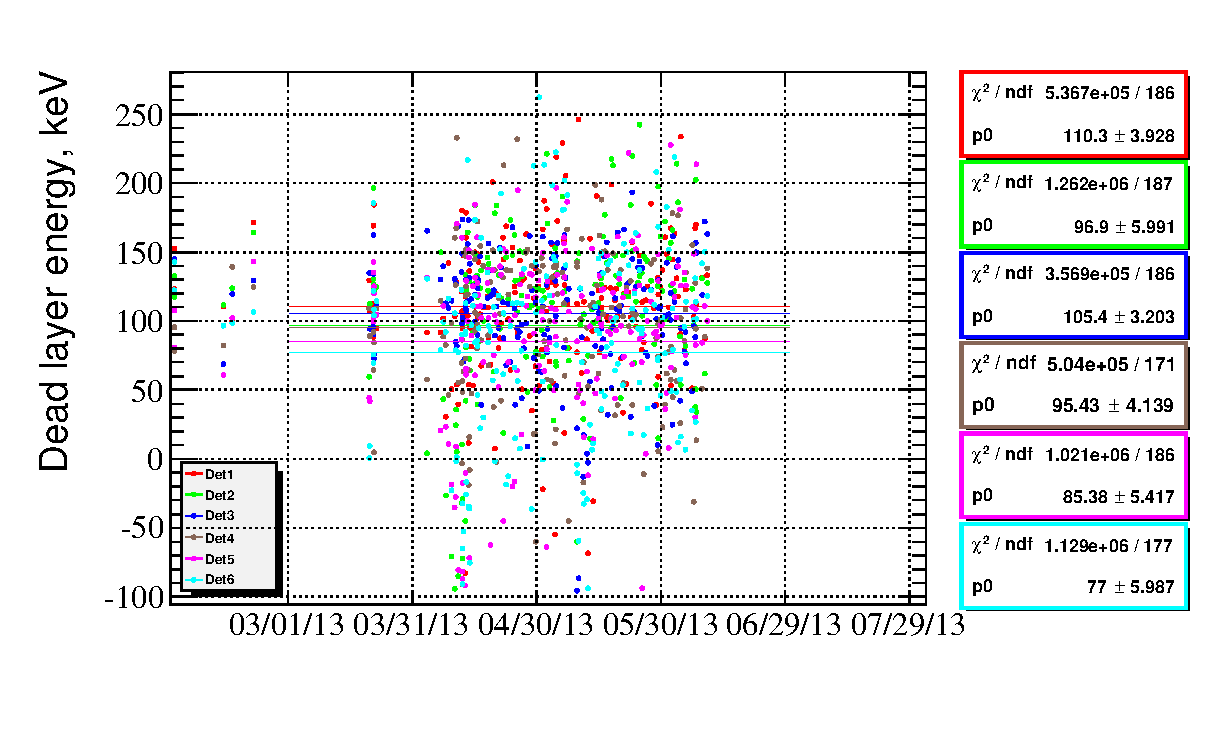
\includegraphics[width=\textwidth]{gfx/run13_alpha_study_novoltagevariation/B2D/c_chDeadLayerEnergy_by_day_B2D.eps}
\caption{B2D}
\end{subfigure}
%
\begin{subfigure}[b]{0.5\textwidth}
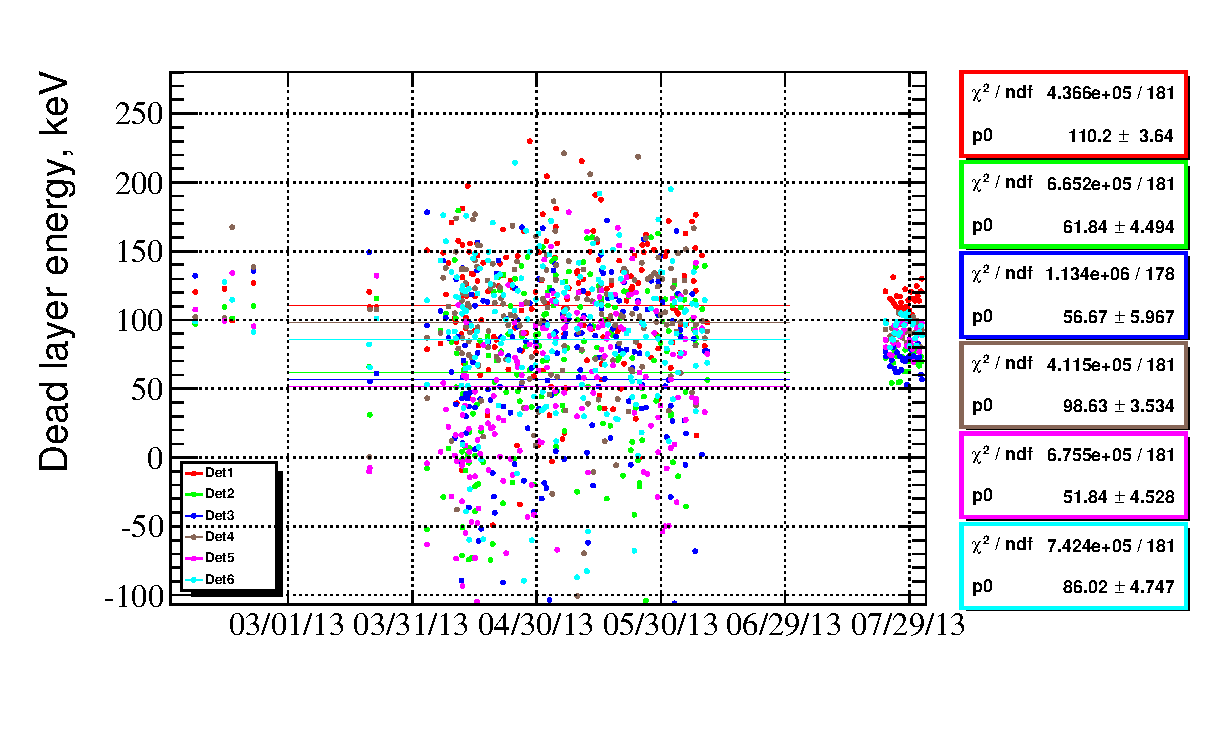
\includegraphics[width=\textwidth]{gfx/run13_alpha_study_novoltagevariation/Y2U/c_chDeadLayerEnergy_by_day_Y2U.eps}
\caption{Y2U}
\end{subfigure}
%
\caption{\edllabellabel{}}
\label{fig:e_dl}
\end{figure}

\newcommand\xdllabel{$x_{DL}$ is the effective dead layer thickness calculated using formula (\ref{eq:x_dl}).}
\begin{figure}
\begin{subfigure}[b]{0.5\textwidth}
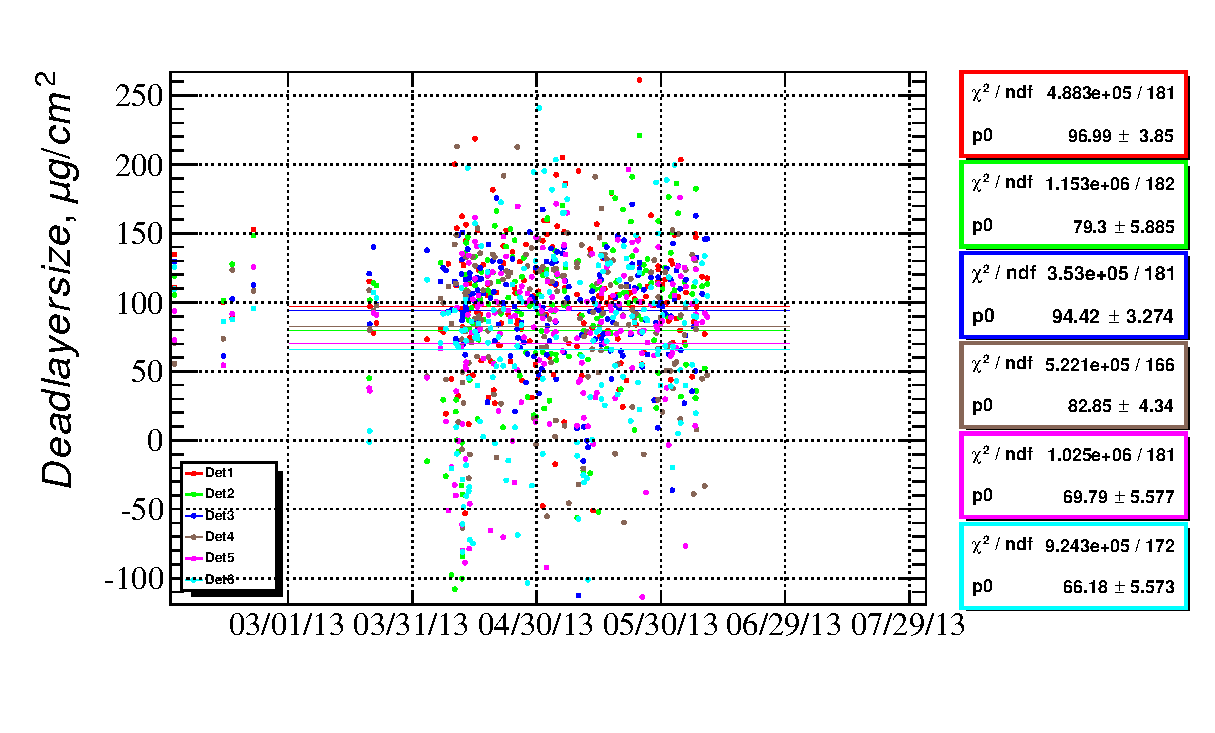
\includegraphics[width=\textwidth]{gfx/run13_alpha_study_novoltagevariation/B2D/c_chDeadLayerSize_by_day_B2D.eps}
\caption{B2D}
\end{subfigure}
%
\begin{subfigure}[b]{0.5\textwidth}
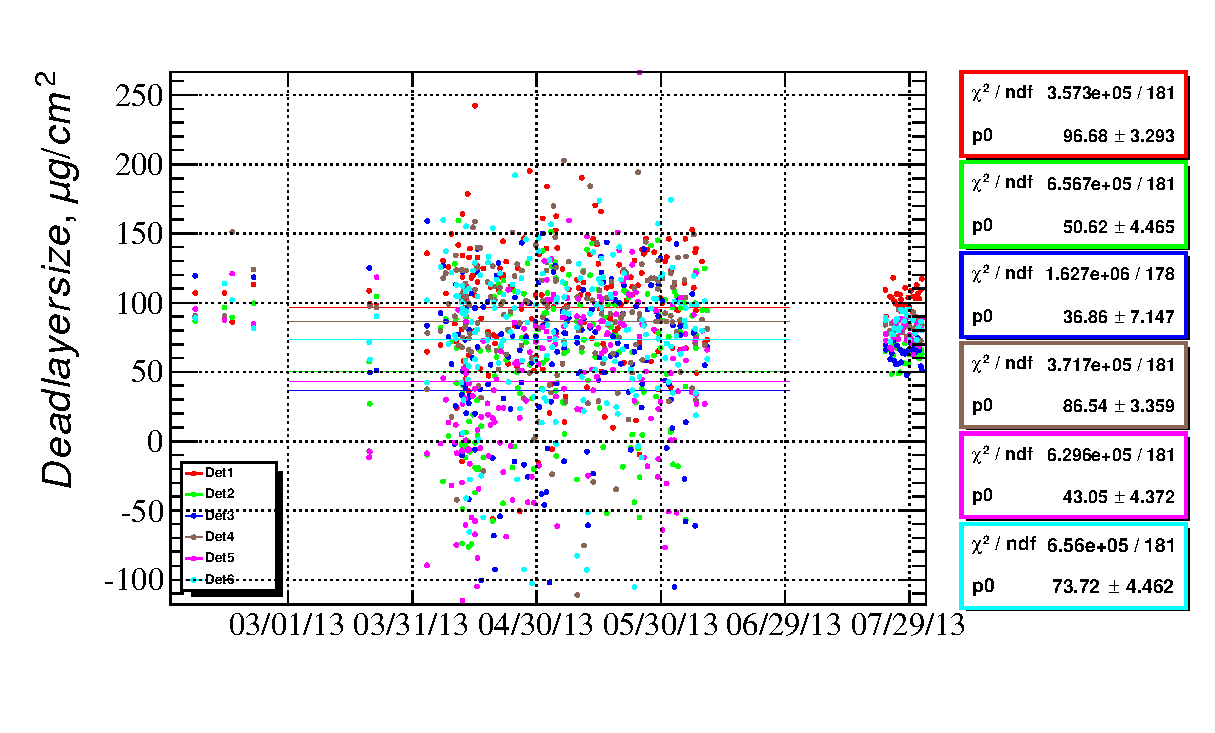
\includegraphics[width=\textwidth]{gfx/run13_alpha_study_novoltagevariation/Y2U/c_chDeadLayerSize_by_day_Y2U.eps}
\caption{Y2U}
\end{subfigure}
\caption{\xdllabel{}}
\label{fig:x_dl}
\end{figure}

\begin{figure}
\begin{subfigure}[b]{0.325\textwidth}
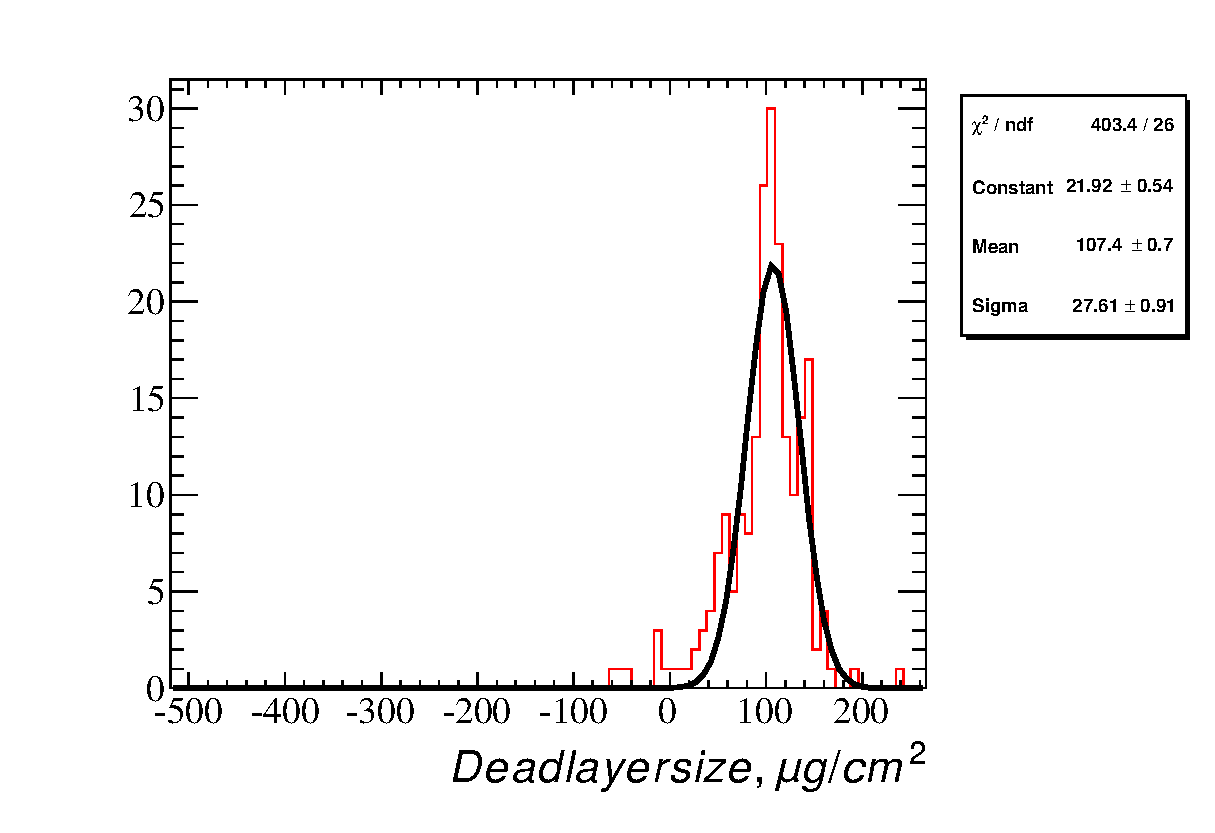
\includegraphics[width=\textwidth]{gfx/run13_alpha_study_novoltagevariation/Y2U/c_hDeadLayerSize_by_run_distribution1_Y2U.eps}
\caption{Det1}
\end{subfigure}
\hfill
\begin{subfigure}[b]{0.325\textwidth}
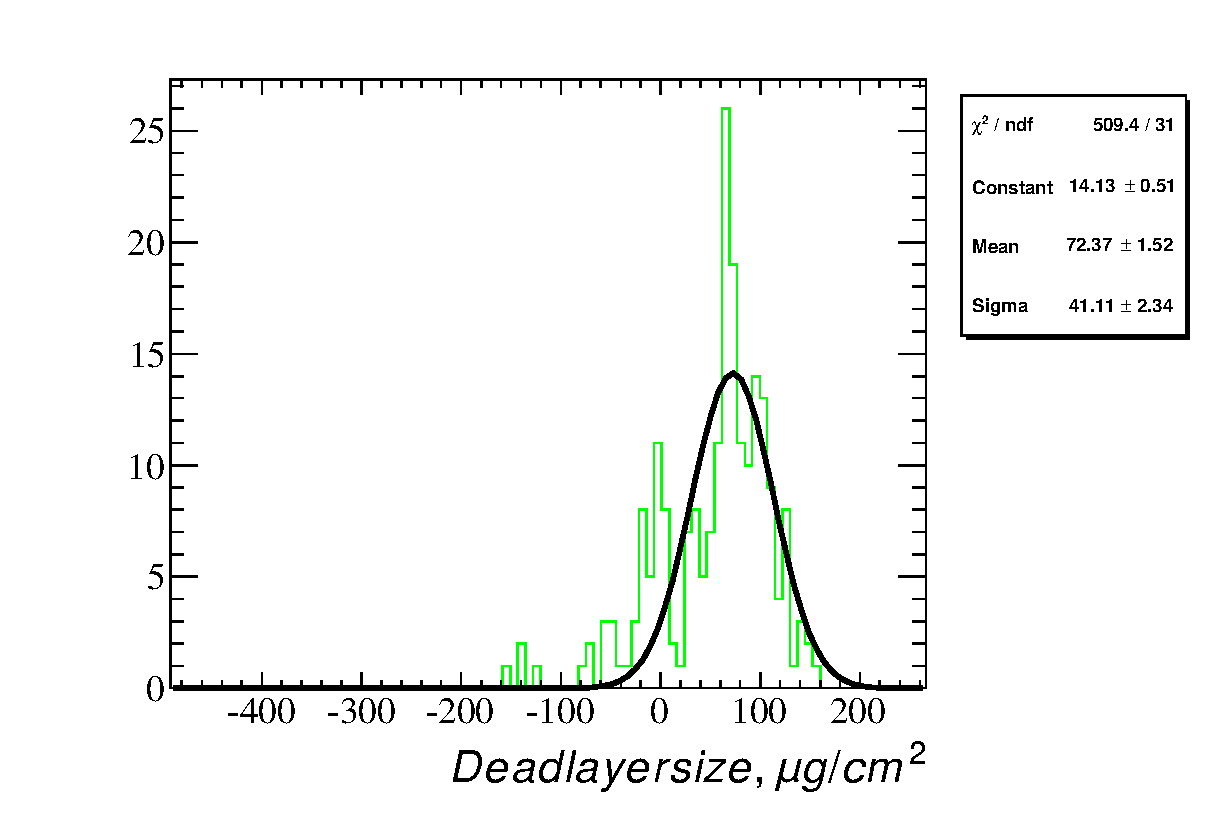
\includegraphics[width=\textwidth]{gfx/run13_alpha_study_novoltagevariation/Y2U/c_hDeadLayerSize_by_run_distribution2_Y2U.eps}
\caption{Det2}
\end{subfigure}
\hfill
\begin{subfigure}[b]{0.325\textwidth}
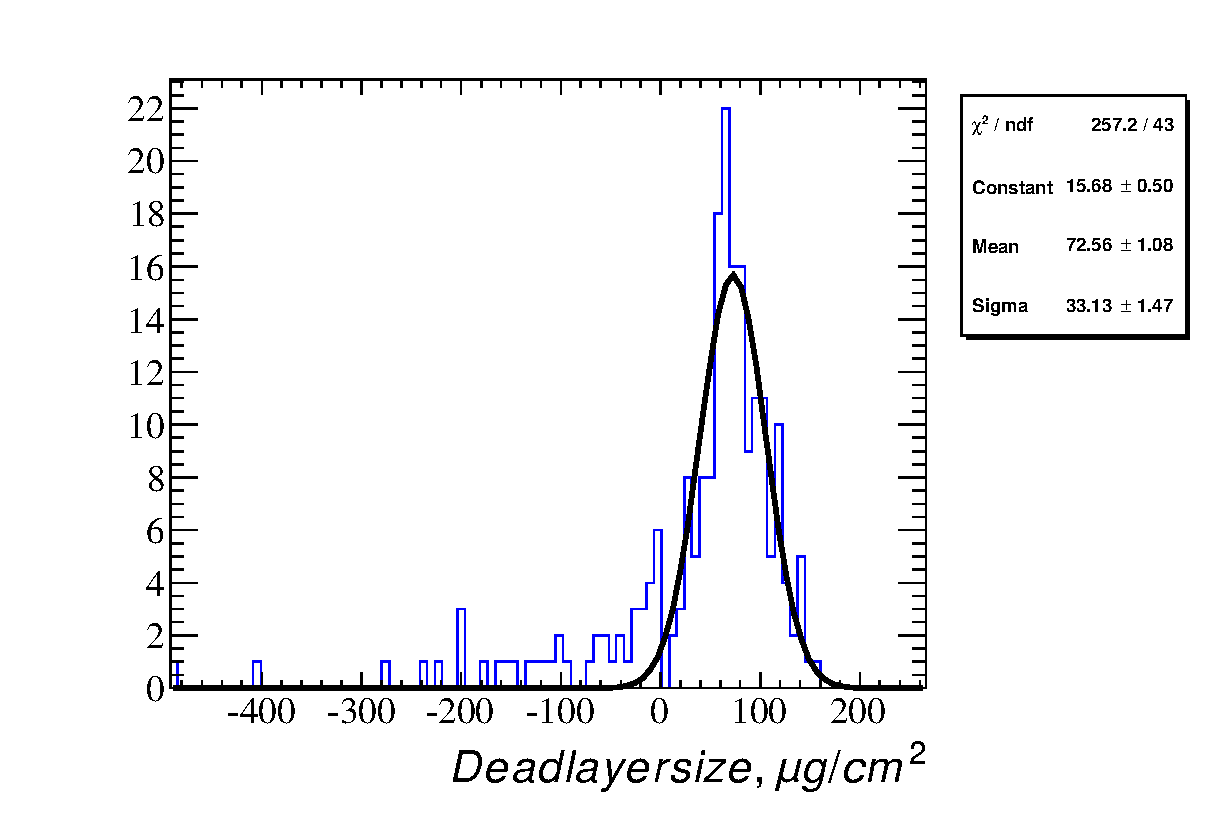
\includegraphics[width=\textwidth]{gfx/run13_alpha_study_novoltagevariation/Y2U/c_hDeadLayerSize_by_run_distribution3_Y2U.eps}
\caption{Det3}
\end{subfigure}
\begin{subfigure}[b]{0.325\textwidth}
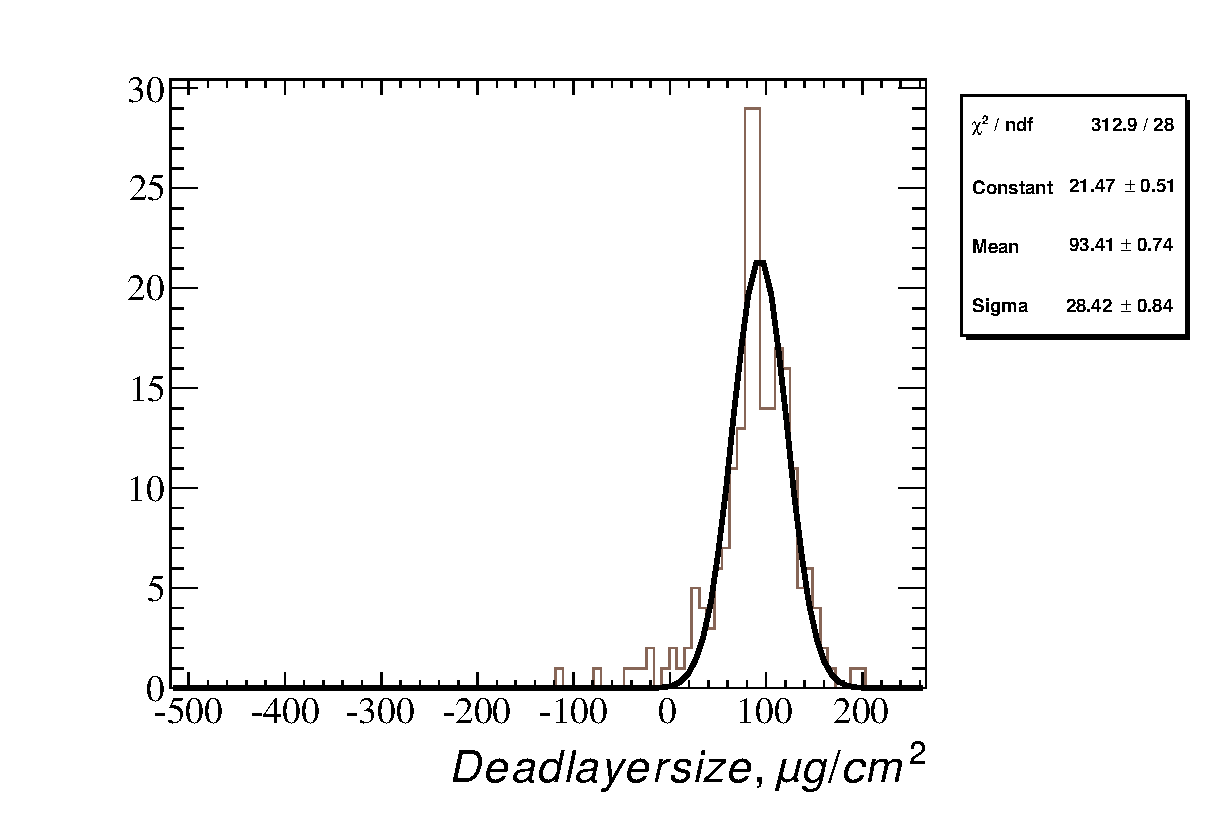
\includegraphics[width=\textwidth]{gfx/run13_alpha_study_novoltagevariation/Y2U/c_hDeadLayerSize_by_run_distribution4_Y2U.eps}
\caption{Det4}
\end{subfigure}
\hfill
\begin{subfigure}[b]{0.325\textwidth}
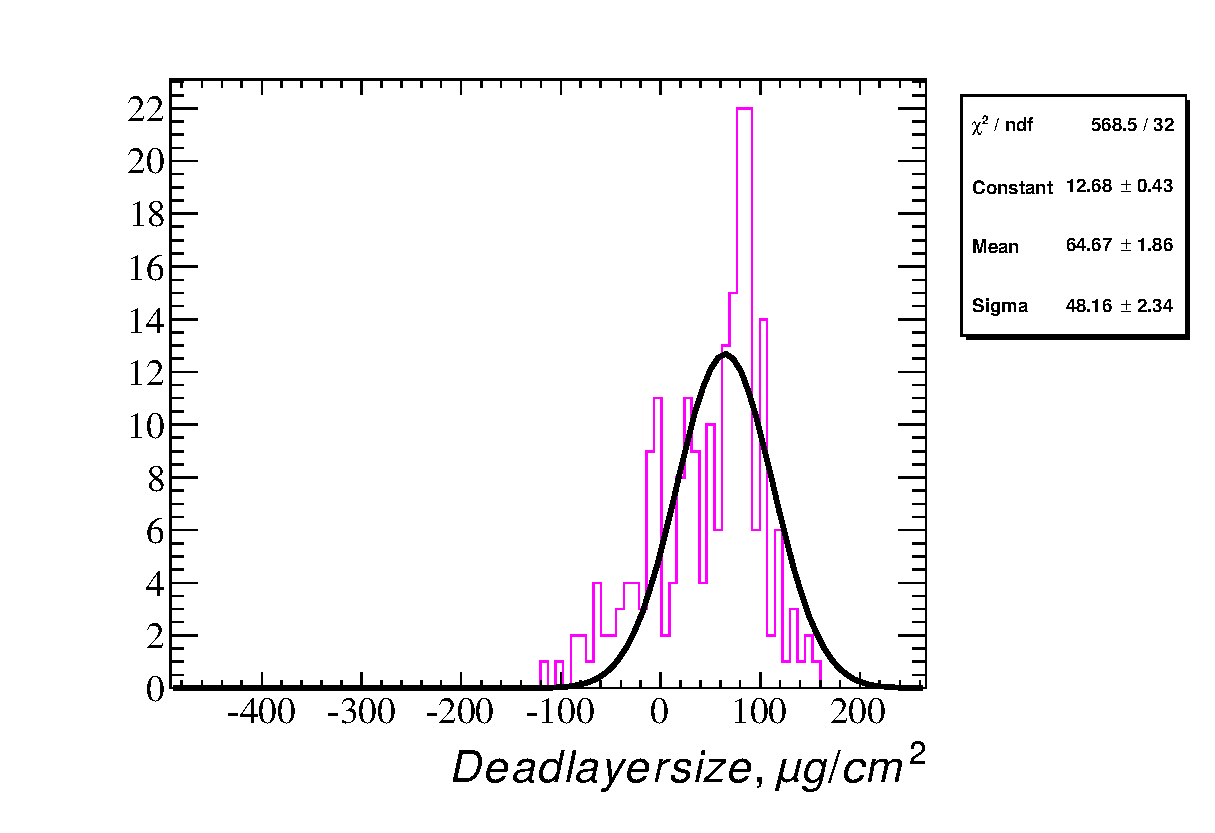
\includegraphics[width=\textwidth]{gfx/run13_alpha_study_novoltagevariation/Y2U/c_hDeadLayerSize_by_run_distribution5_Y2U.eps}
\caption{Det5}
\end{subfigure}
\hfill
\begin{subfigure}[b]{0.325\textwidth}
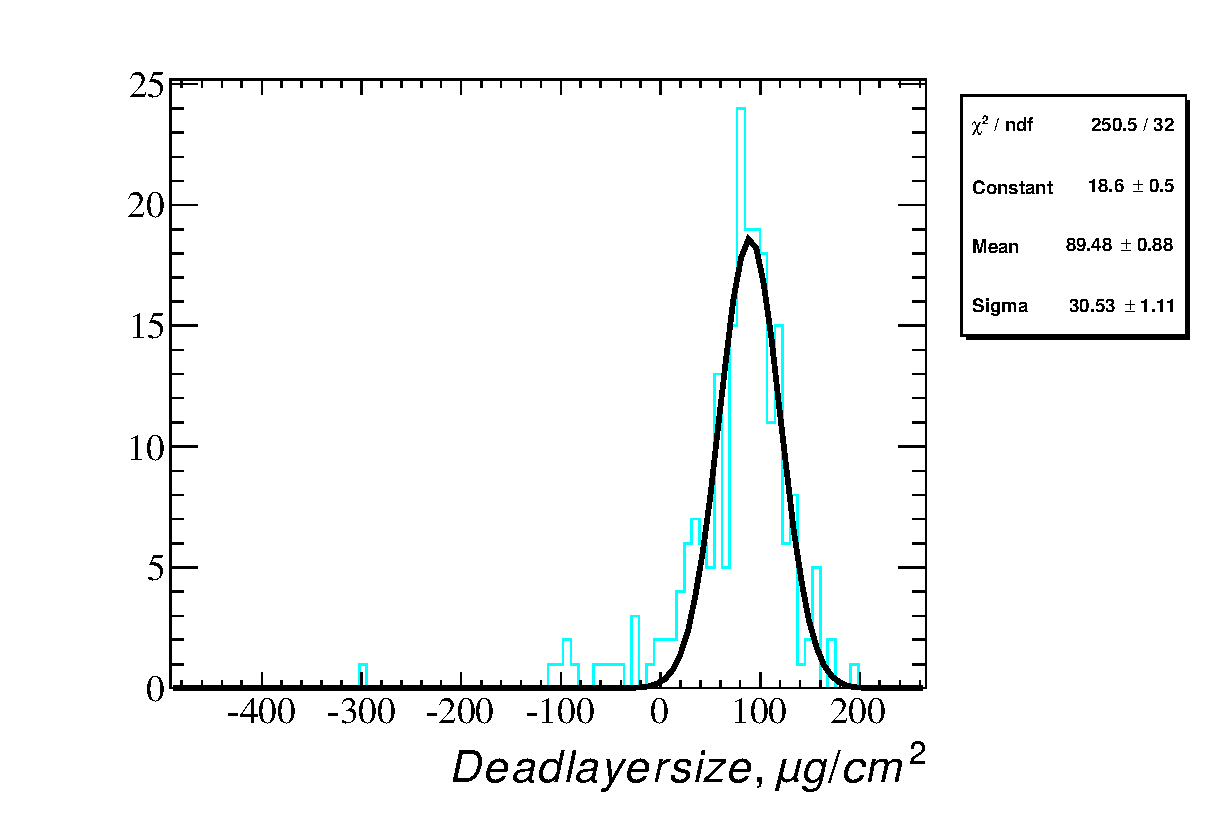
\includegraphics[width=\textwidth]{gfx/run13_alpha_study_novoltagevariation/Y2U/c_hDeadLayerSize_by_run_distribution6_Y2U.eps}
\caption{Det6}
\end{subfigure}
\caption{$x_{DL}$ distribution in the measurements for Y2U.}
\end{figure}
\begin{figure}
\begin{subfigure}[b]{0.325\textwidth}
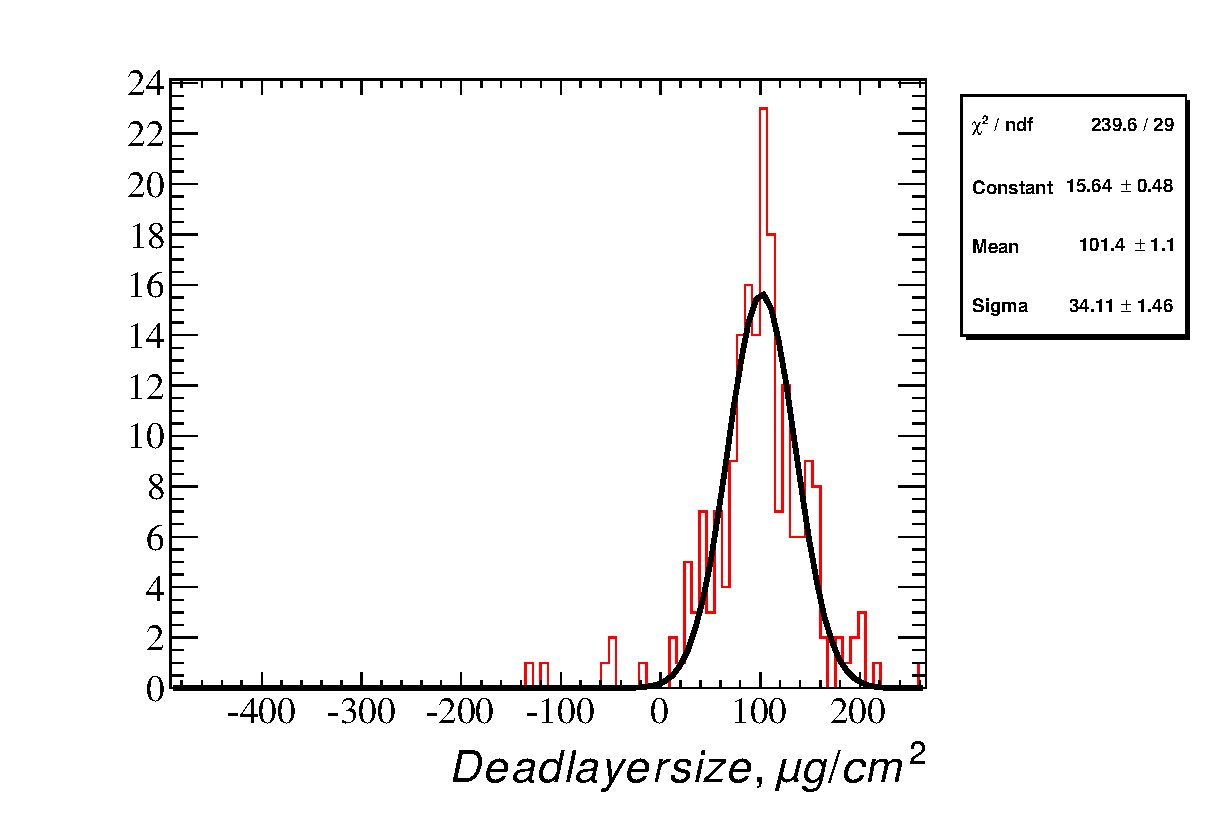
\includegraphics[width=\textwidth]{gfx/run13_alpha_study_novoltagevariation/B2D/c_hDeadLayerSize_by_run_distribution1_B2D.eps}
\caption{Det1}
\end{subfigure}
\hfill
\begin{subfigure}[b]{0.325\textwidth}
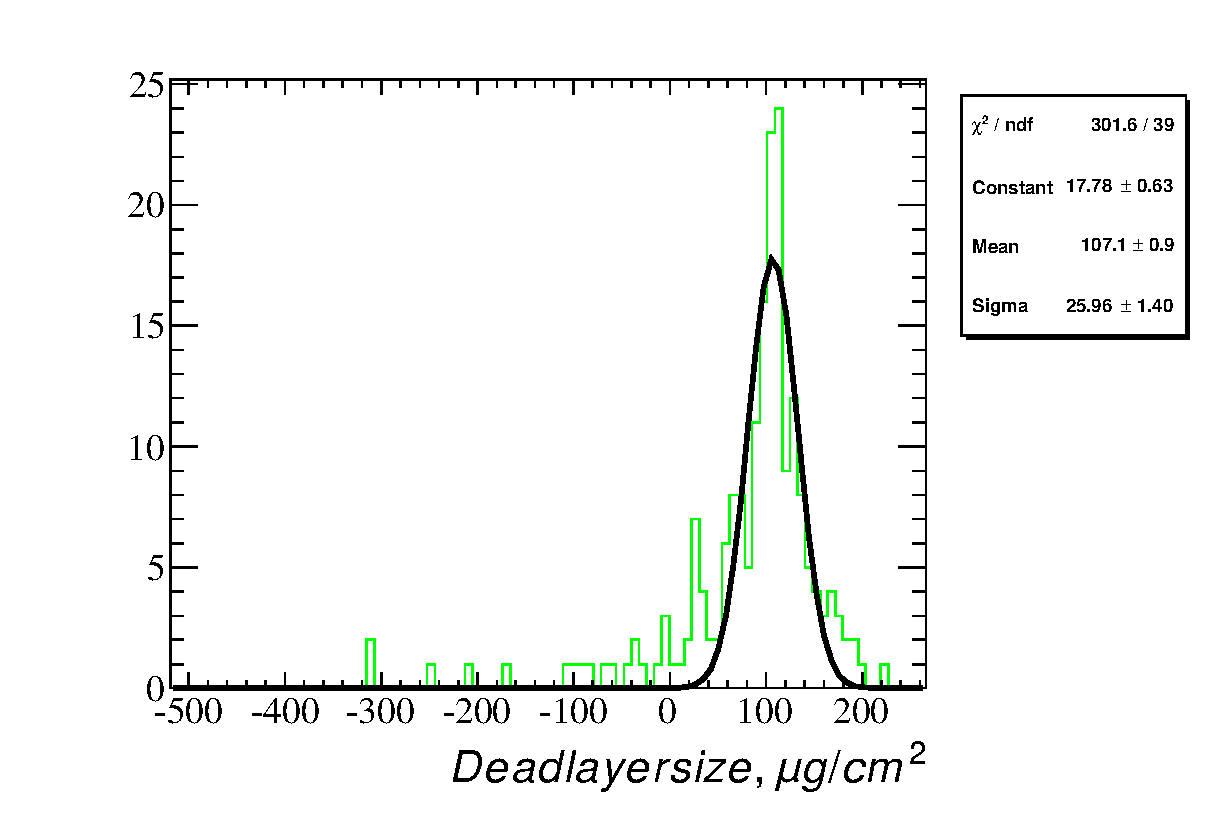
\includegraphics[width=\textwidth]{gfx/run13_alpha_study_novoltagevariation/B2D/c_hDeadLayerSize_by_run_distribution2_B2D.eps}
\caption{Det2}
\end{subfigure}
\hfill
\begin{subfigure}[b]{0.325\textwidth}
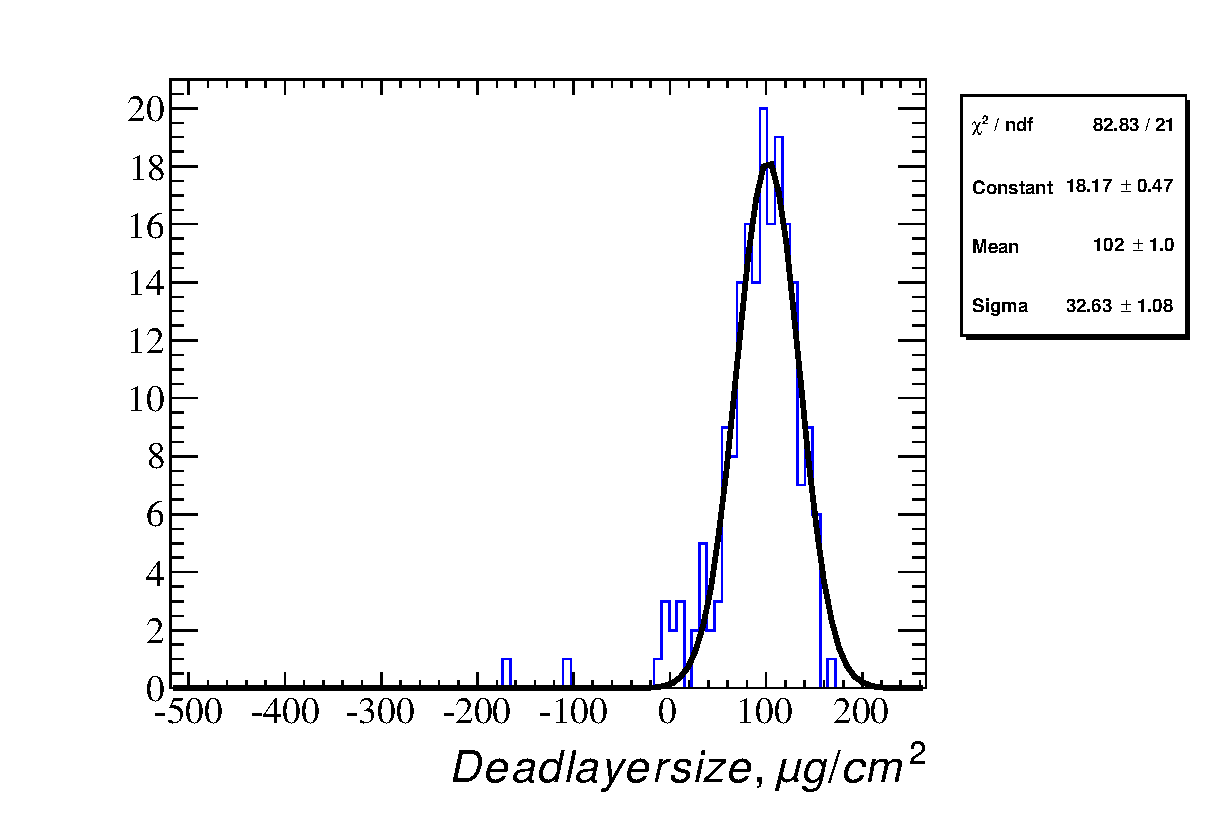
\includegraphics[width=\textwidth]{gfx/run13_alpha_study_novoltagevariation/B2D/c_hDeadLayerSize_by_run_distribution3_B2D.eps}
\caption{Det3}
\end{subfigure}
\begin{subfigure}[b]{0.325\textwidth}
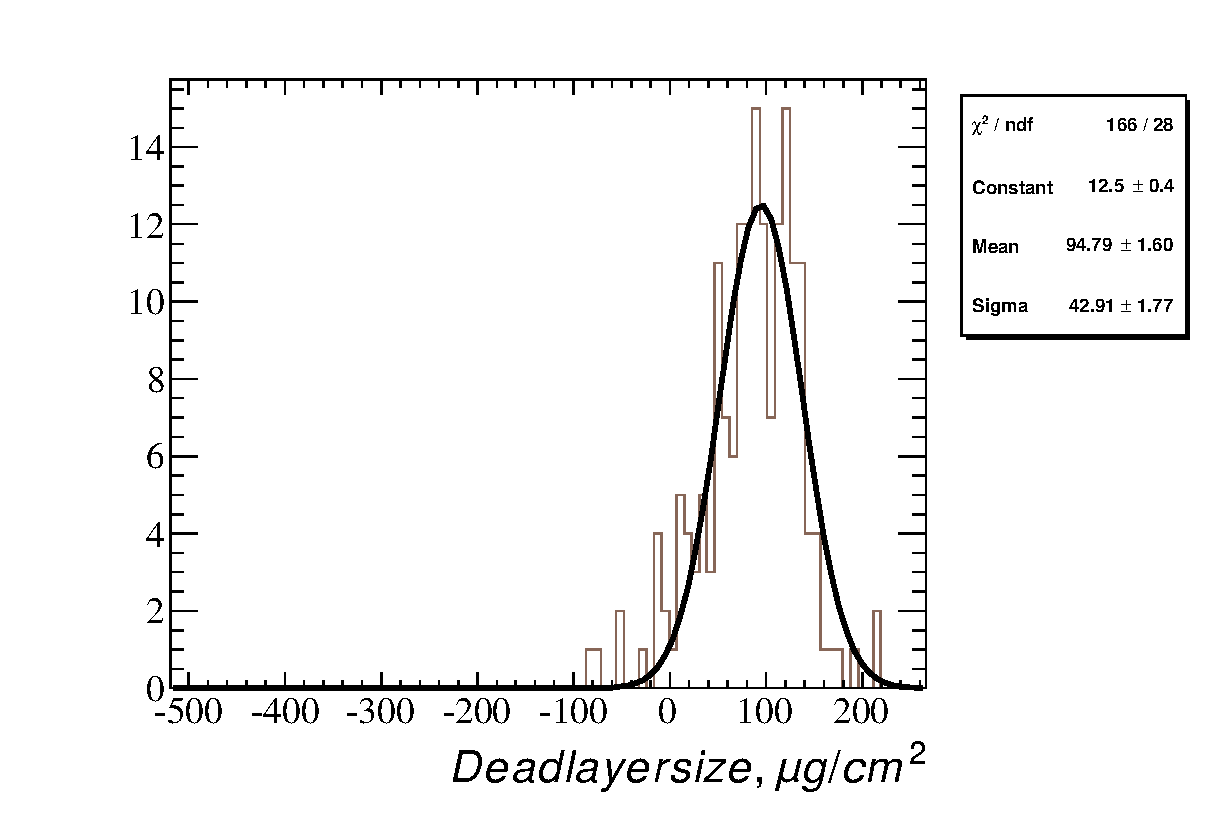
\includegraphics[width=\textwidth]{gfx/run13_alpha_study_novoltagevariation/B2D/c_hDeadLayerSize_by_run_distribution4_B2D.eps}
\caption{Det4}
\end{subfigure}
\hfill
\begin{subfigure}[b]{0.325\textwidth}
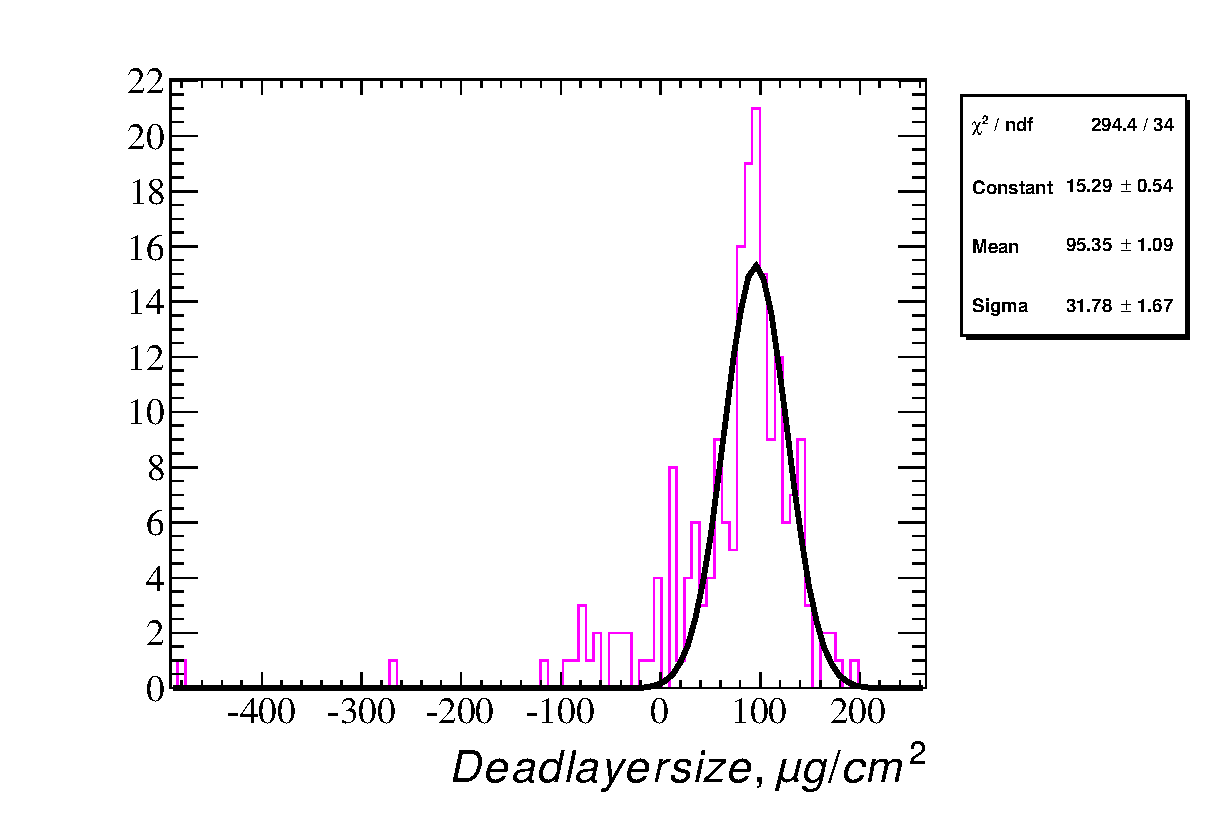
\includegraphics[width=\textwidth]{gfx/run13_alpha_study_novoltagevariation/B2D/c_hDeadLayerSize_by_run_distribution5_B2D.eps}
\caption{Det5}
\end{subfigure}
\hfill
\begin{subfigure}[b]{0.325\textwidth}
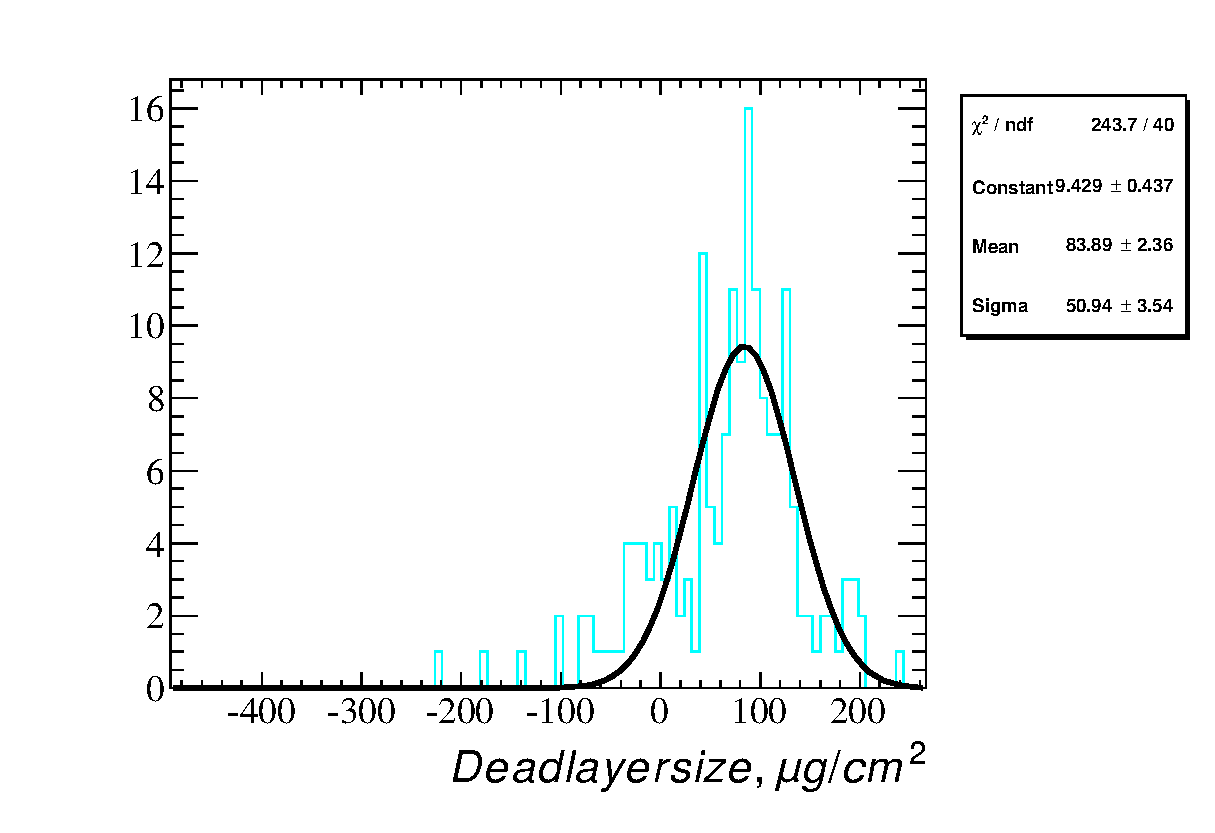
\includegraphics[width=\textwidth]{gfx/run13_alpha_study_novoltagevariation/B2D/c_hDeadLayerSize_by_run_distribution6_B2D.eps}
\caption{Det6}
\end{subfigure}
\caption{$x_{DL}$ distribution in the measurements for B2D.}
\end{figure}

\subsection{Bias current}

% TODO: write something about how out bias current varies over time

In \cref{fig:gain_relations,fig:e_dl,fig:x_dl} there are few measurements taken
before and after run13. When comparing these measurements with the measurements
taken during the run we see that later are showing much higher spread.  We
investigate this abnormality by looking at correlations with other
detector work parameters.

One of the work parameters of our silicon detector that we measure is a bias
current -- current constantly flowing through detector (in this case -- set of
12 strips). Current was measured for each of the six silicon detectors on all
polarimeters, measurements were taken each five minutes. Values lie mostly in
range from $-30$ to $0$~$\mu\text{A}$. It was interesting to see how this current
affects calibration characteristics of our detector. For example, it is known
that higher bias voltage should decrease size of depleted zone, i.e. decrease
size of effective dead layer. On our plots (\cref{fig:bc_vs_xdl}) we see some weak
correlation between effective dead layer size and bias current.

\newcommand\bcvsxdllabel{Bias current versus dead layer size dependency.}
\begin{figure}
\begin{subfigure}[t]{0.5\textwidth}
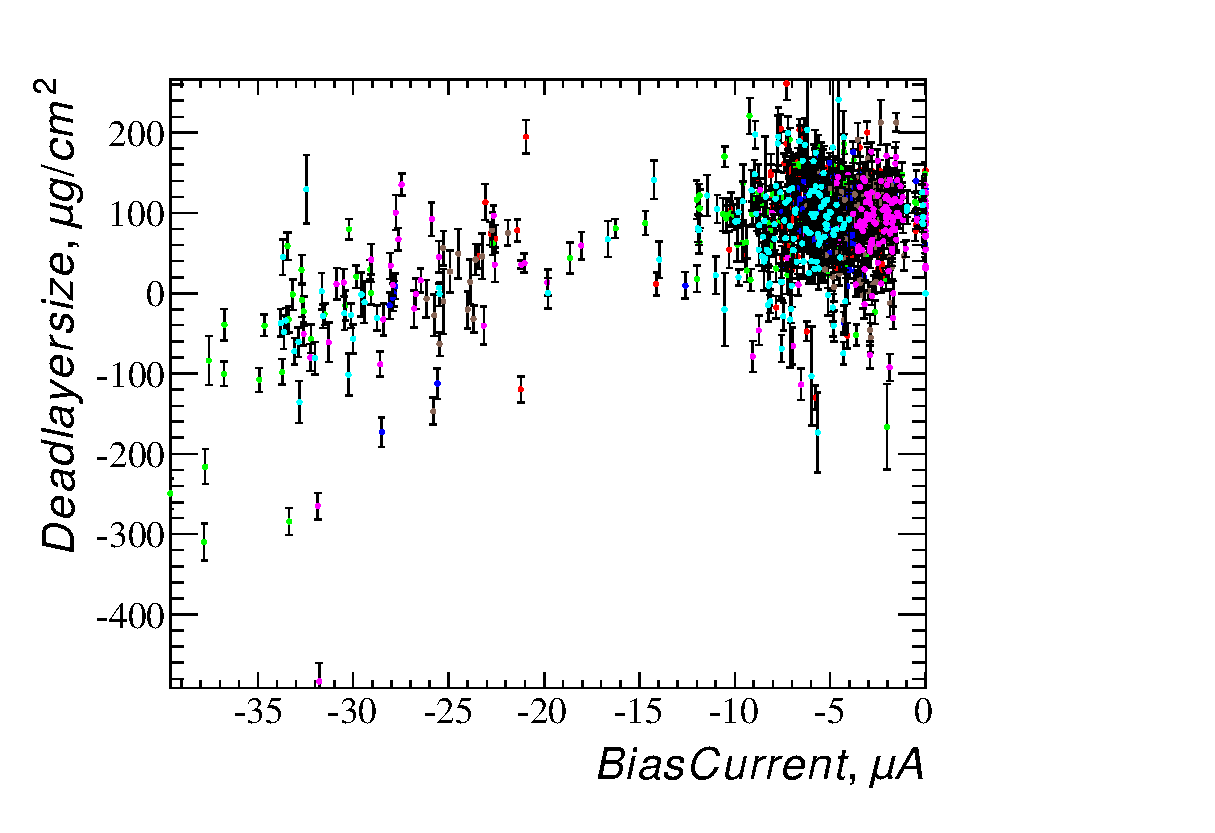
\includegraphics[width=\textwidth]{gfx/run13_alpha_study_novoltagevariation/B2D/c_hBiasCurrent_DeadLayerSize.eps}
\caption{B2D}
\end{subfigure}
%
\begin{subfigure}[t]{0.5\textwidth}
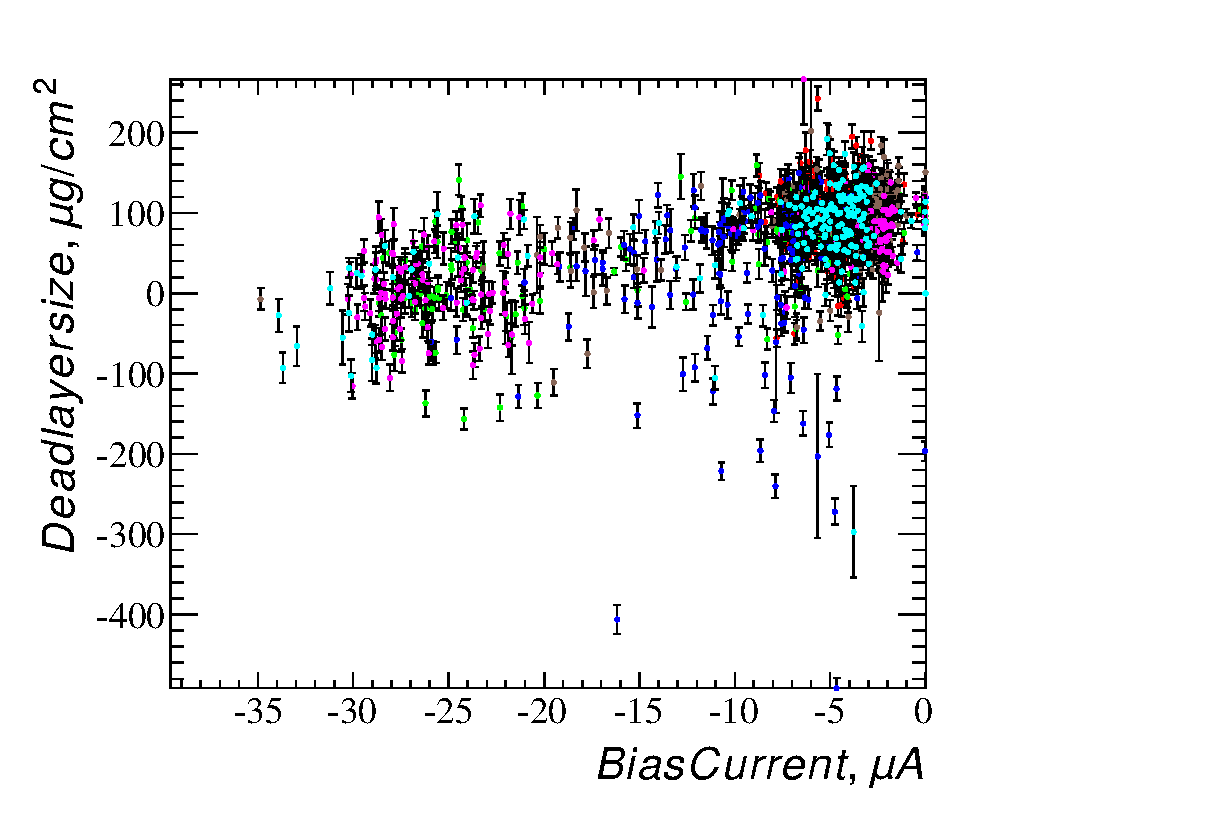
\includegraphics[width=\textwidth]{gfx/run13_alpha_study_novoltagevariation/Y2U/c_hBiasCurrent_DeadLayerSize.eps}
\caption{Y2U}
\end{subfigure}
\caption{\bcvsxdllabel{}}
\label{fig:bc_vs_xdl}
\end{figure}

Much stronger correlation is seen when we compare the bias current with the
gain (\cref{fig:bc_vs_gain}). We use this correlation to produce linear model
to correct our alpha gains to their values at zero bias current. The resulting
plot is presented at \cref{fig:gainAmCorrected}. Unlike original plot at
\cref{fig:gainAmCorrected} this one shows much lower spread.

We assume that presented dependence of alpha gain on bias current holds true
during the sweep measurements. Study of the dependence of carbon energy
spectrum slope over bias current
\cite{schmidke_alpha_vs_carbon}\cite{dkalinkin_bc_vs_carbongain} shows that
this is likely to be true in our case. As we see in \cref{fig:bc_jumping} the
bias current may change very quickly during the fill, what should cause changes
to the effective alpha gain.  Correction similar to the one described in the
previous paragraph should be then applied.


\newcommand\bcvsgainlabel{Bias current versus americium gain ($\mu_{\text{Am}} /
E_{\text{Am}}$) dependency. The colors represent different detectors.}
\begin{figure}
\begin{subfigure}[b]{0.5\textwidth}
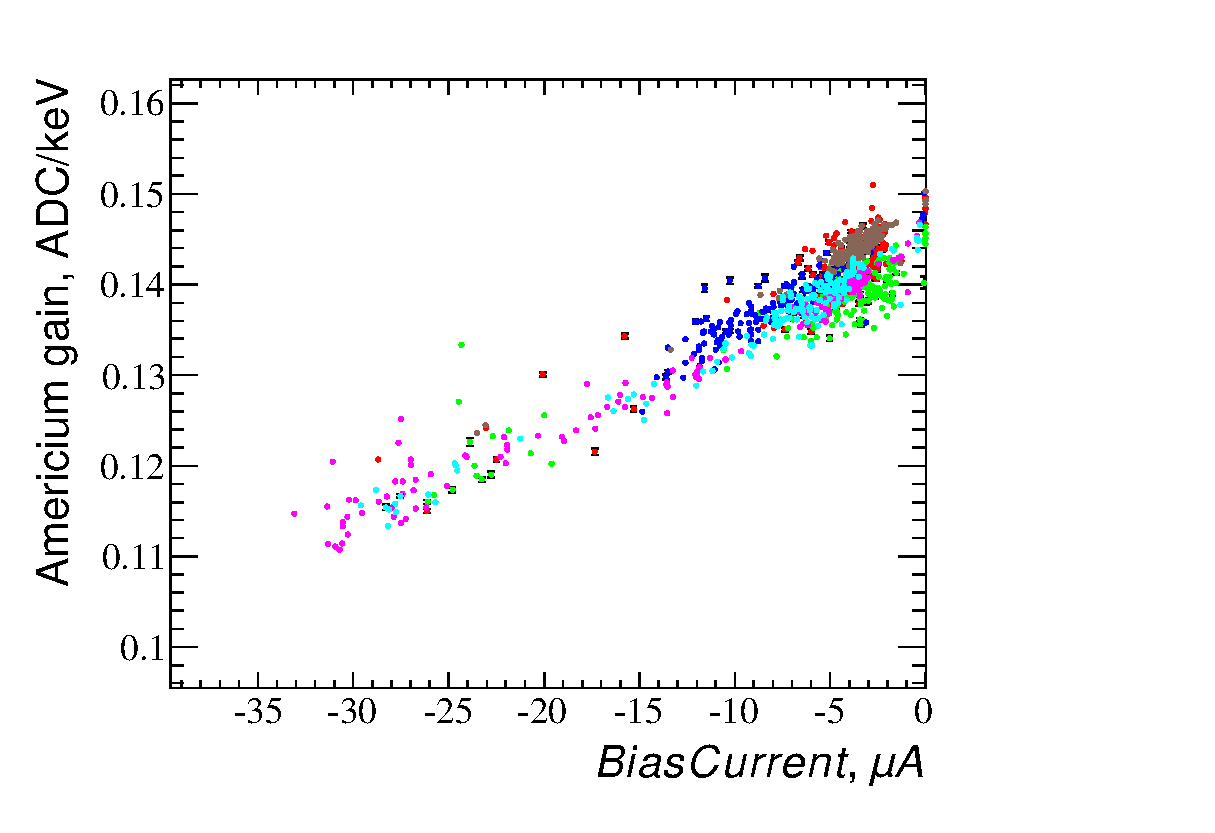
\includegraphics[width=\textwidth]{gfx/run13_alpha_study_novoltagevariation/B1U/c_hBiasCurrent_AmGain.eps}
\caption{B1U}\label{bc_vs_gain-b1u}
\end{subfigure}
\begin{subfigure}[b]{0.5\textwidth}
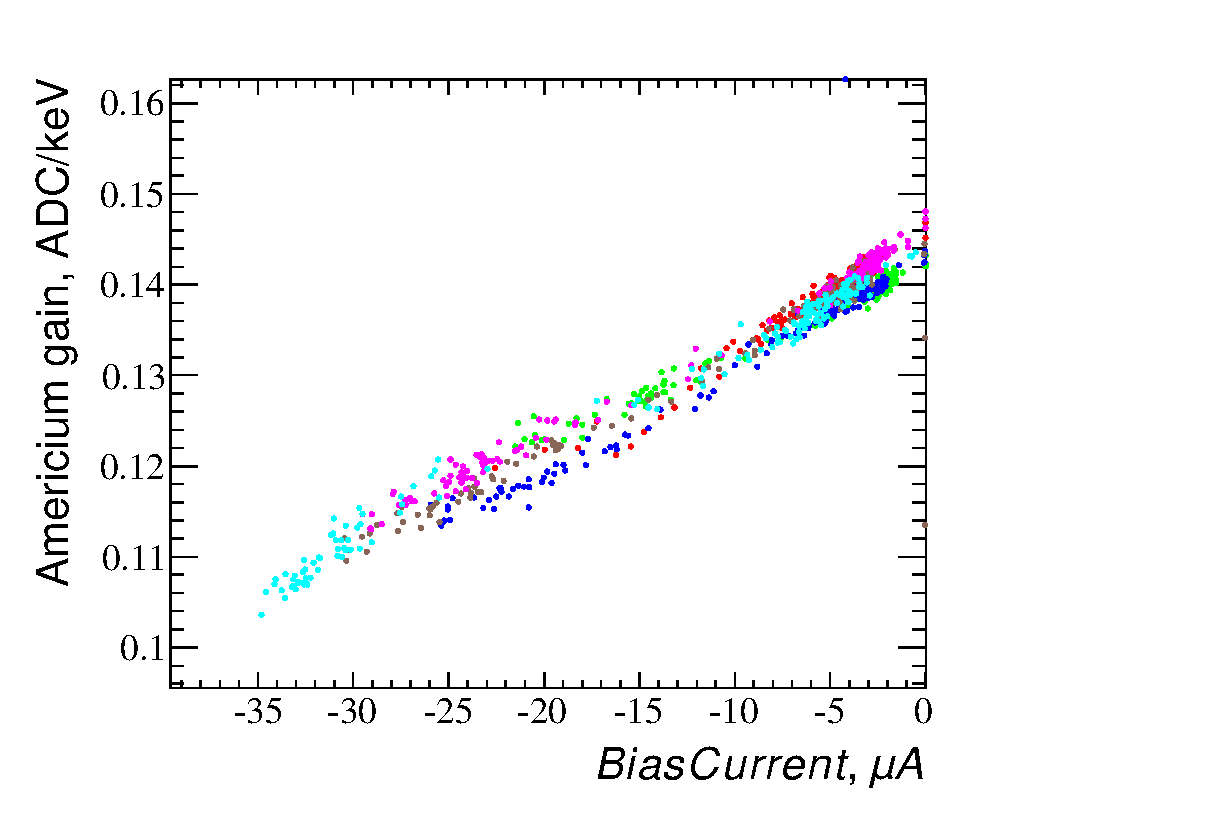
\includegraphics[width=\textwidth]{gfx/run13_alpha_study_novoltagevariation/Y1D/c_hBiasCurrent_AmGain.eps}
\caption{Y1D}\label{bc_vs_gain-y1d}
\end{subfigure}

\begin{subfigure}[b]{0.5\textwidth}
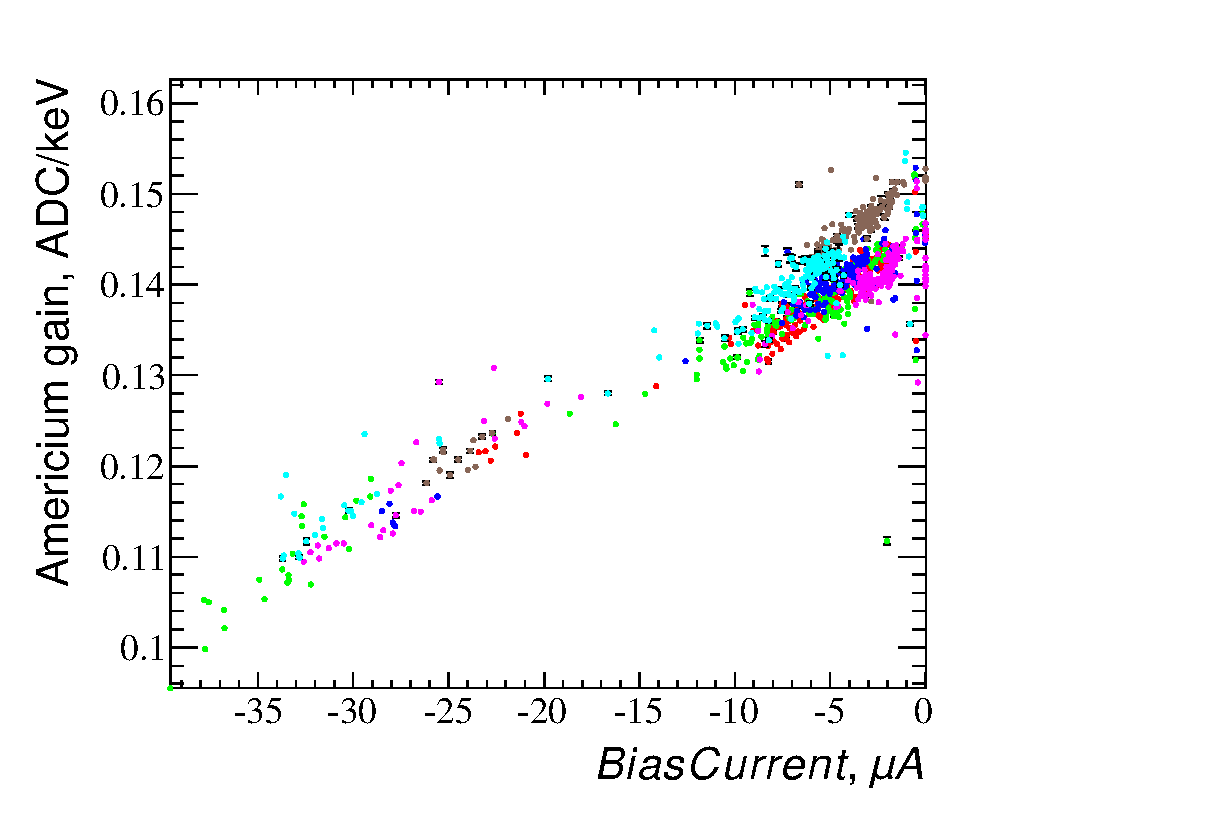
\includegraphics[width=\textwidth]{gfx/run13_alpha_study_novoltagevariation/B2D/c_hBiasCurrent_AmGain.eps}
\caption{B2D}\label{bc_vs_gain-b2d}
\end{subfigure}
\begin{subfigure}[b]{0.5\textwidth}
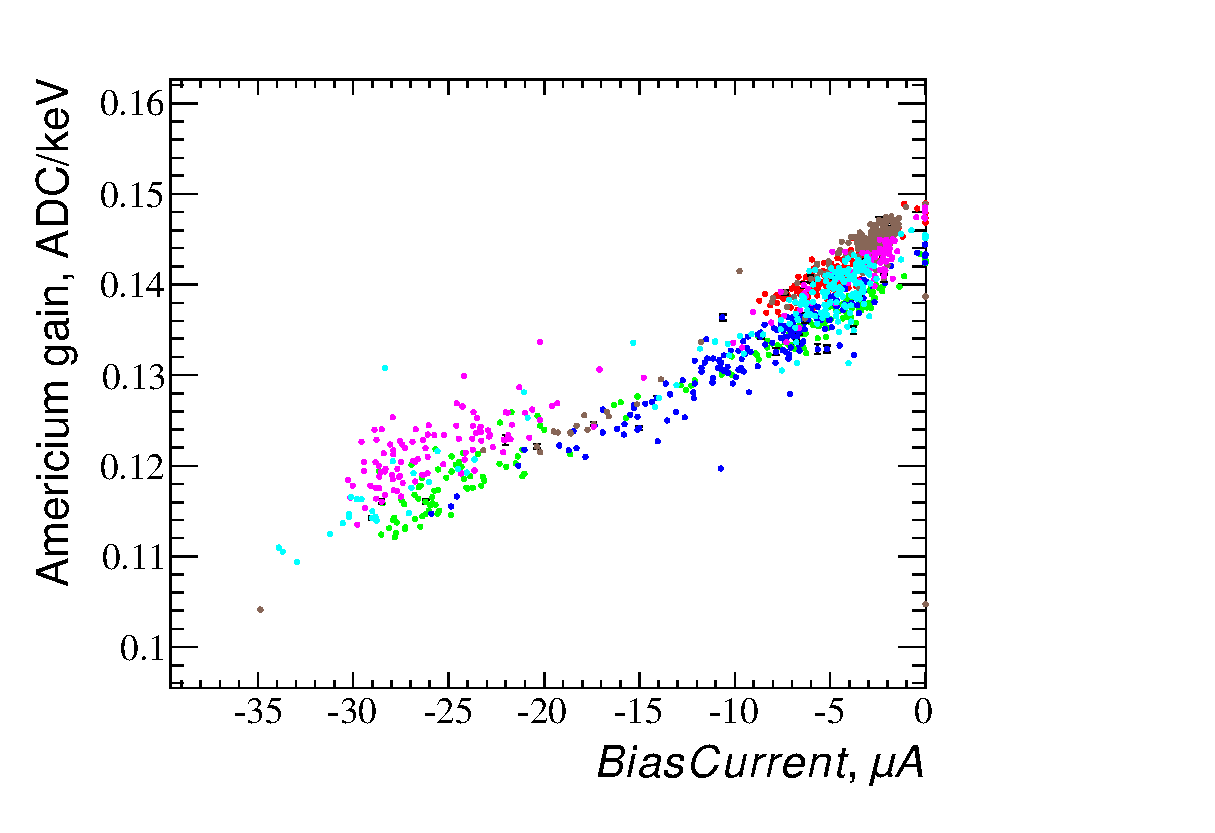
\includegraphics[width=\textwidth]{gfx/run13_alpha_study_novoltagevariation/Y2U/c_hBiasCurrent_AmGain.eps}
\caption{Y2U}\label{bc_vs_gain-y2u}
\end{subfigure}

\caption{\bcvsgainlabel{}}
\label{fig:bc_vs_gain}
\end{figure}

\begin{figure}
%
\begin{subfigure}[t]{0.49\textwidth}
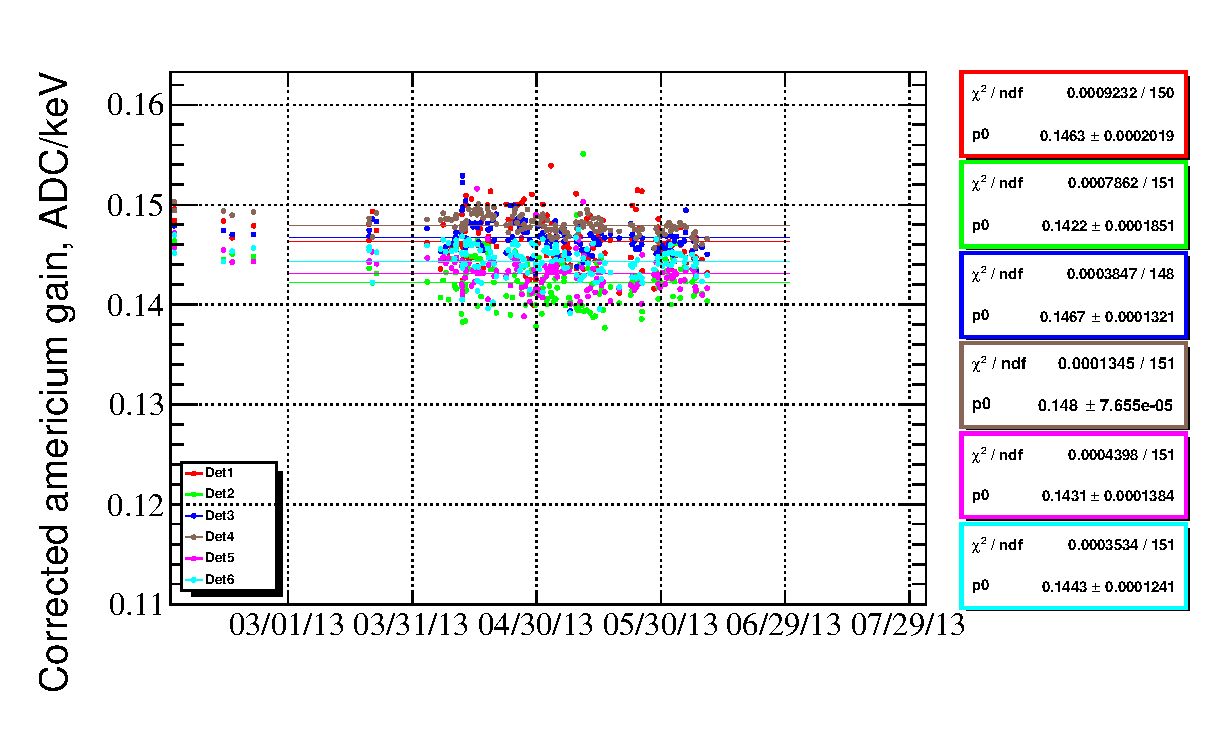
\includegraphics[width=\textwidth]{gfx/run13_alpha_study_novoltagevariation/B1U/c_chAmGainCorrected_by_day_B1U.eps}
\caption{B1U}
\end{subfigure}
%
\hfill
%
\begin{subfigure}[t]{0.49\textwidth}
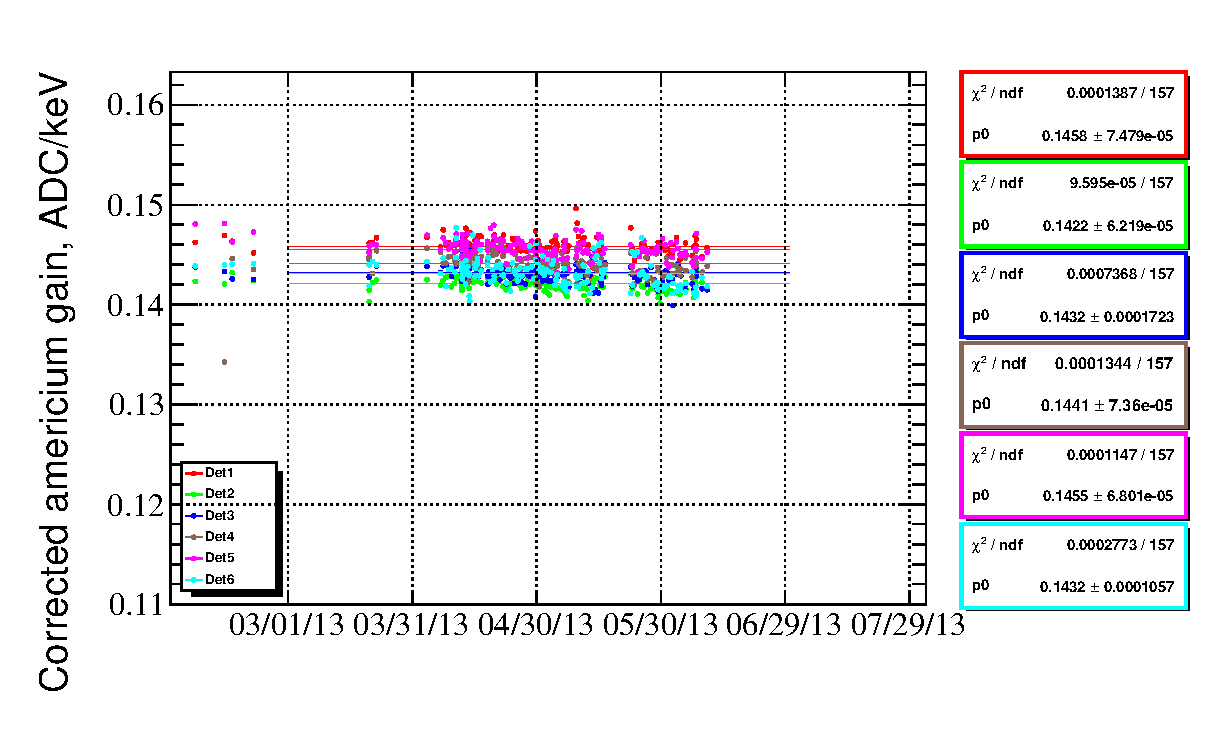
\includegraphics[width=\textwidth]{gfx/run13_alpha_study_novoltagevariation/Y1D/c_chAmGainCorrected_by_day_Y1D.eps}
\caption{Y1D}
\end{subfigure}
%
\begin{subfigure}[t]{0.49\textwidth}
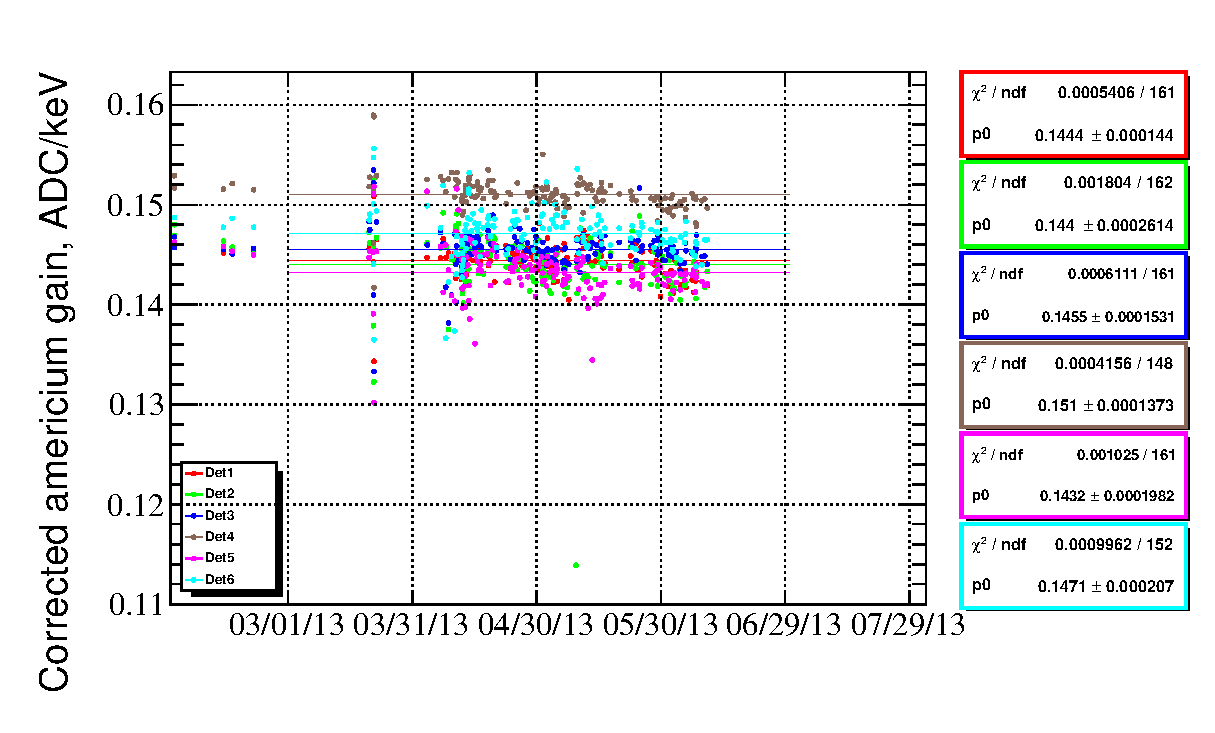
\includegraphics[width=\textwidth]{gfx/run13_alpha_study_novoltagevariation/B2D/c_chAmGainCorrected_by_day_B2D.eps}
\caption{B2D}
\end{subfigure}
%
\hfill
%
\begin{subfigure}[t]{0.49\textwidth}
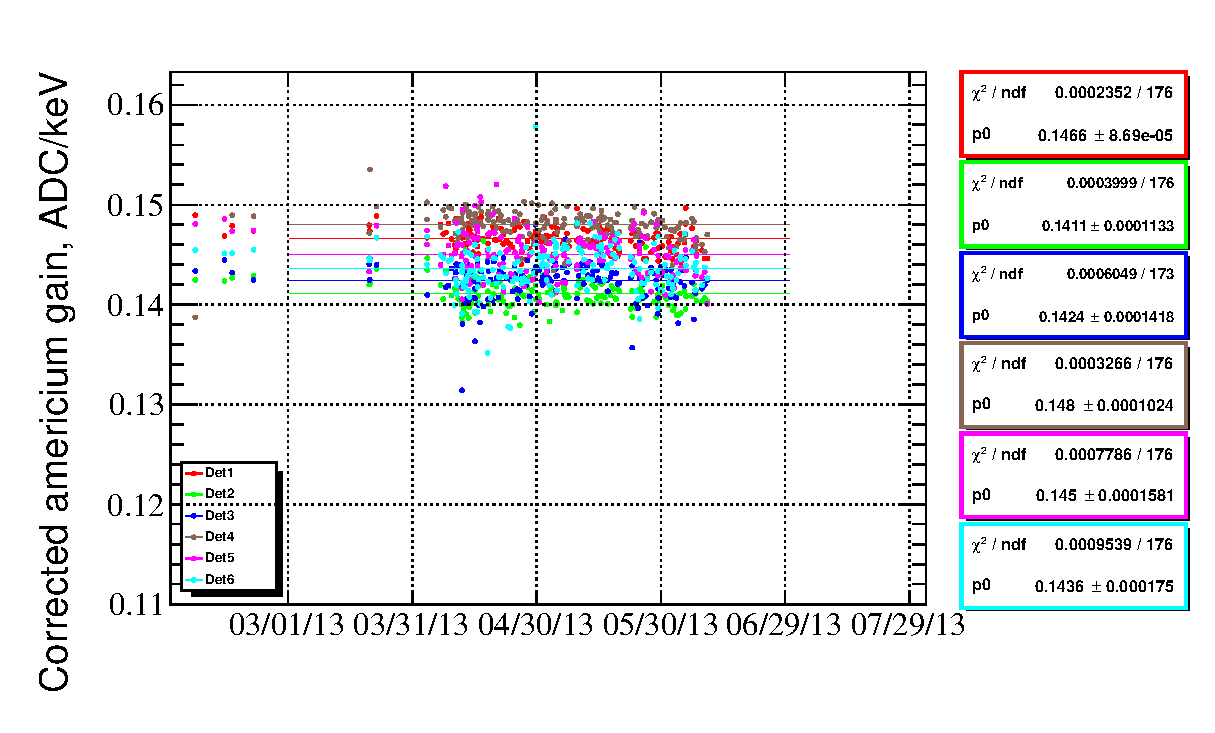
\includegraphics[width=\textwidth]{gfx/run13_alpha_study_novoltagevariation/Y2U/c_chAmGainCorrected_by_day_Y2U.eps}
\caption{Y2U}
\end{subfigure}
%
\caption{Time dependence of the detector gain $g_\text{Am}$ that was corrected
to zero bias current using the slope from \cref{fig:bc_vs_gain}.}
\label{fig:gainAmCorrected}
\end{figure}

We also tried to see if the variation of the bias current correlates with the
beam properties. To do that we took average of the beam intensity values at a
plateau (values $> 50 \cdot 10^{11}$ protons) of the fill happened before the
alpha measurement. That value was then plotted versus the bias current as
shown at \cref{fig:bc_vs_beamcurrent}.

\begin{figure}
\begin{subfigure}[t]{0.5\textwidth}
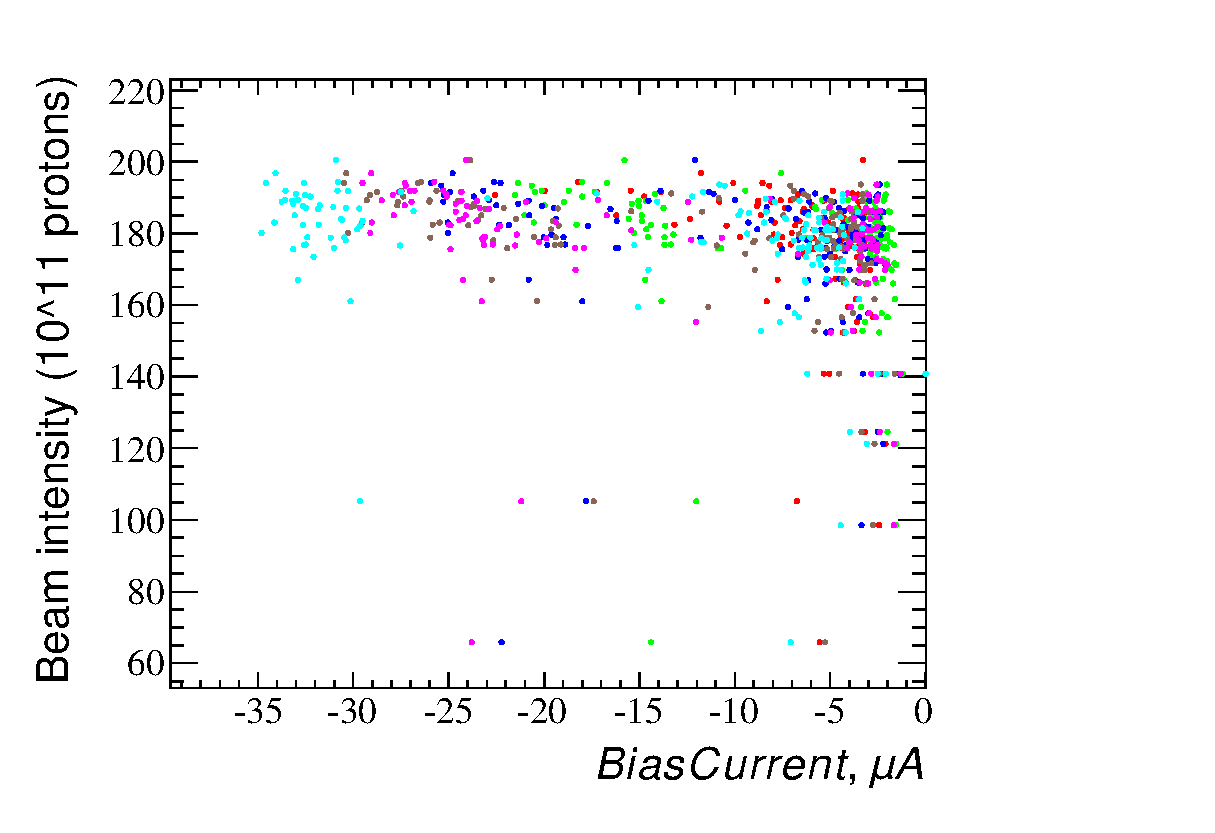
\includegraphics[width=\textwidth]{gfx/run13_alpha_study_novoltagevariation/Y1D/c_hBiasCurrent_BeamCurrent.eps}
\caption{Y1D}
\end{subfigure}
%
\begin{subfigure}[t]{0.5\textwidth}
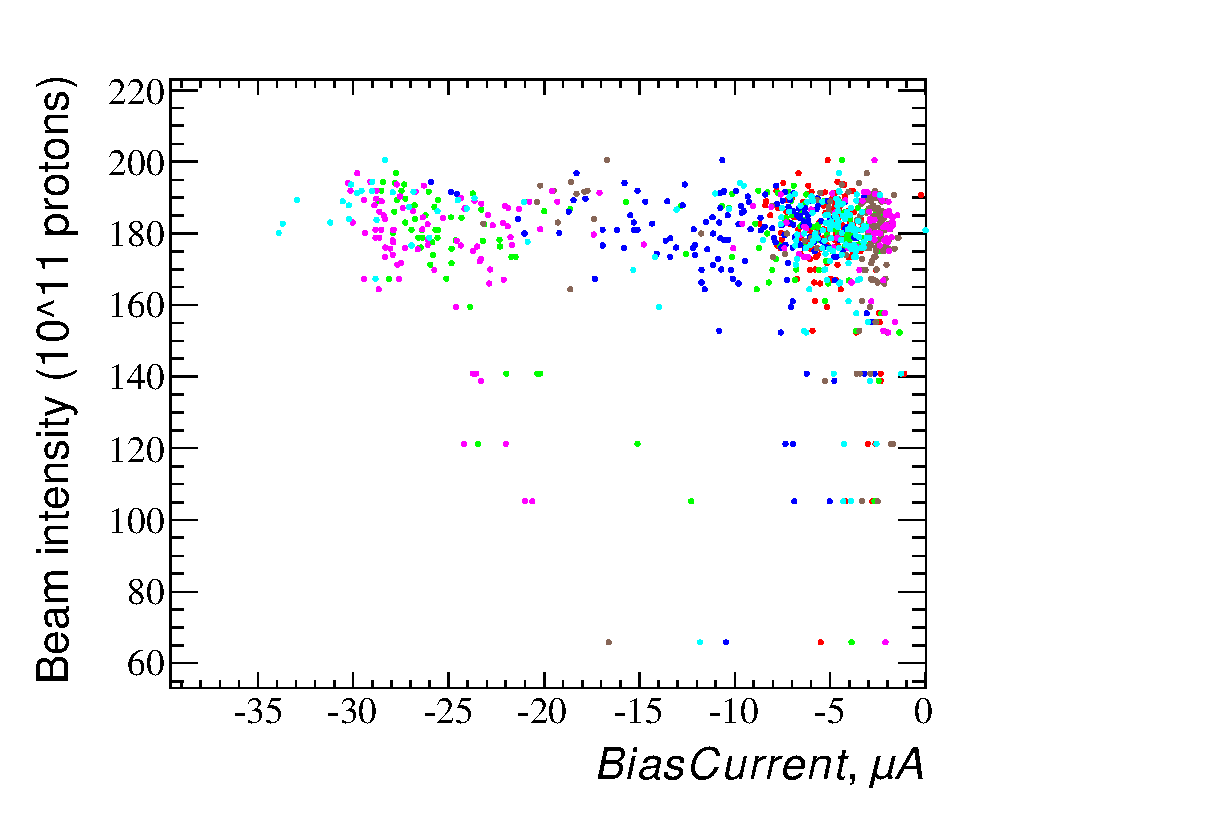
\includegraphics[width=\textwidth]{gfx/run13_alpha_study_novoltagevariation/Y2U/c_hBiasCurrent_BeamCurrent.eps}
\caption{Y2U}
\end{subfigure}
%
\caption{The average bias current during an alpha measurement versus the average
beam intensity in the preceding store. The colors represent different
detectors.}
\label{fig:bc_vs_beamcurrent}
\end{figure}

\begin{figure}
\center{
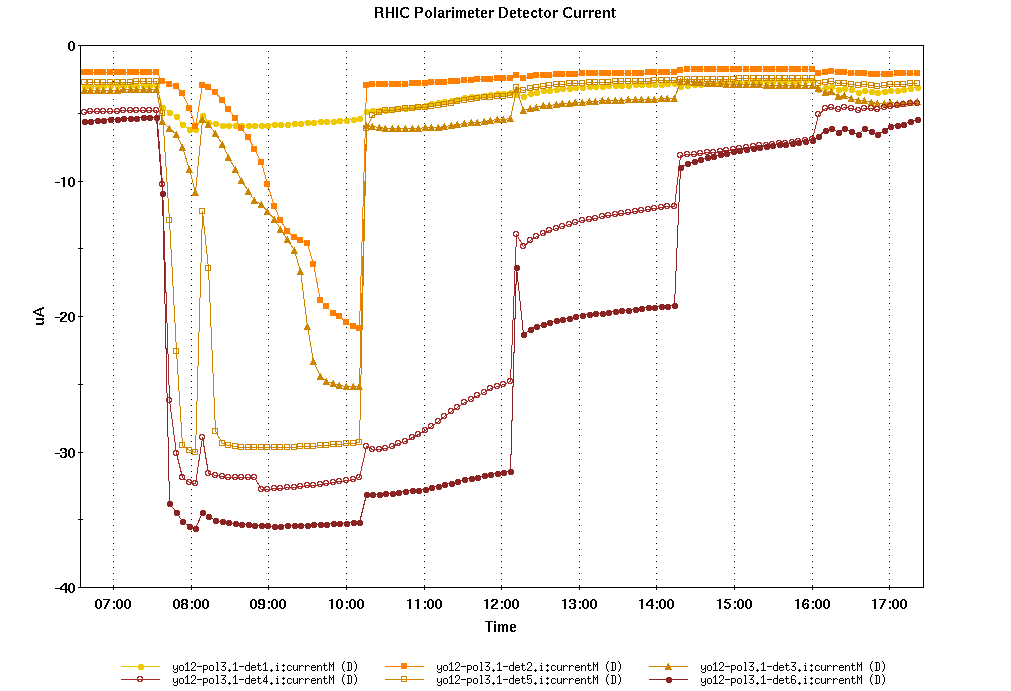
\includegraphics[width=\textwidth]{gfx/bias_current.17384.yel1.png}
}
\caption{Bias current variation in Y1D detector during fill 17384. Some jumps
coincide with polarization measurements.}
\label{fig:bc_jumping}
\end{figure}

\subsection{Linearity of the amplifiers}

The signal generated in the detector propagates through several stages of
amplification. Linearity of the downstream amplifiers can be checked by
attenuating the signal in a place on the signal path preceding the
amplification, and then comparing the measured reduced amplitude with the
expected one properly scaled by a known factor.

The shaper boards have a resistive divider with a multiplexer controlled by
software settings. For normal polarization measurements of sub-MeV carbon ions
the on-board attenuator is set to 1, i.e. no signal attenuation. During regular
alpha measurements the attenuator is set to $1/5$. In this study we check the
other two attenuator settings of $1/10$ and $1/3$. The alpha peaks obtained with
these attenuator settings are shown in \cref{fig:atten_distrib} and the
mean values corresponding to the gaussian fits are listed in
\cref{table:atten}. Note that with the attenuator setting of $1/3$ the
americium peak ends up in the overflow bin as the events are outside of the detector
dynamic range. The cumulative effect of a possible non-linearity in the
amplified signal is checked by using the relation in which the mean of
the peak is expected to scale with the attenuator settings:

\begin{equation}
\lambda_1/\lambda_2 = \mu_1/ \mu_2.
\label{eq:atten_linearity}
\end{equation}


\begin{table}[htb]
\caption{The mean positions of the \americium{} and \gadolinium{} $\alpha$-peaks
with different attenuator settings.}
\centering

\begin{tabular}{clrr}
\toprule
Attenuation $\lambda$ & Alpha Run Id      & Am Mean, ADC      & Gd Mean, ADC \\
\midrule
$\frac{1}{10}$  & \small{atten\_1\_over\_10.yel2.alpha0}  & $77.0\pm0.7$      & $44.2\pm0.4$ \\
\addlinespace
$\frac{1}{5}$   & \small{13\_310713.yel2.alpha0}          & $154.9\pm2.7$     & $88.9\pm1.5$ \\
\addlinespace
$\frac{1}{3}$   & \small{atten\_1\_over\_3.yel2.alpha0}   & ---\hspace{20pt}  & $149.4\pm2.5$ \\
\bottomrule
\end{tabular}

\label{table:atten}
\end{table}

\noindent
This effect relative to one of the attenuator settings can be defined as
$\Delta l = \frac{\lambda_1 \mu_2}{\lambda_2 \mu_1} - 1$. For the three pairs
of measurements we calculate very small deviations from the linear
\cref{eq:atten_linearity}.

\begin{equation}
\frac{154.9}{77.0 \times 2} - 1 = 0.6\%
\qquad
\frac{88.9}{44.0 \times 2} - 1 = 0.6\%
\qquad
\frac{149.4 \times 3}{88.9 \times 5} - 1 = 0.8\%
\end{equation}


\begin{figure}[htb]
\centering
\begin{subfigure}[t]{0.49\textwidth}
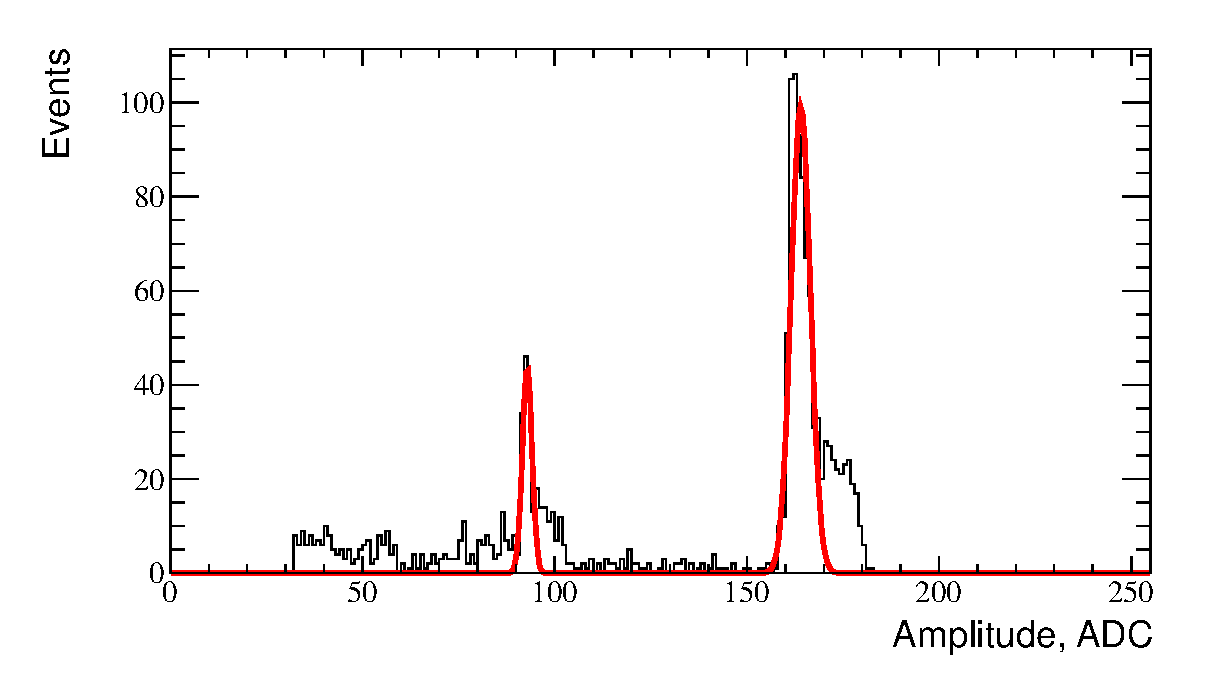
\includegraphics[width=\textwidth]{gfx/atten_1_over_5_ch06.eps}
\caption{Signal attenuated to $1/5$}
\label{fig:atten_distrib_nominal}
\end{subfigure}

\begin{subfigure}[t]{0.49\textwidth}
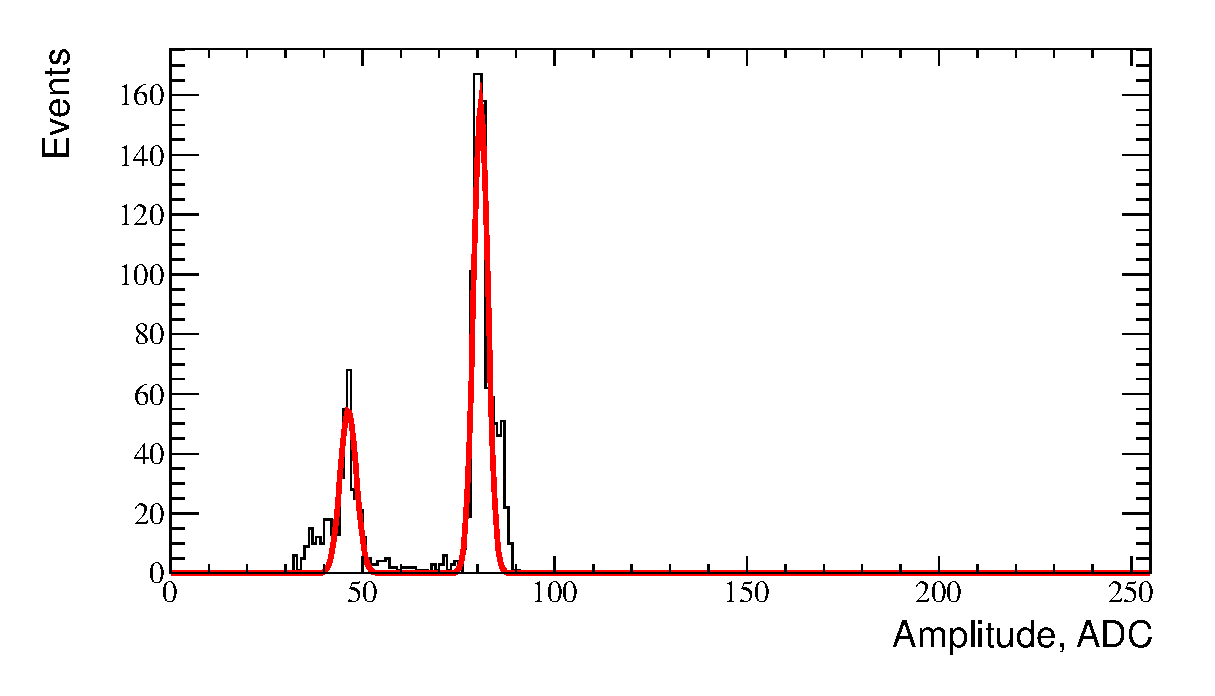
\includegraphics[width=\textwidth]{gfx/atten_1_over_10_ch06.eps}
\caption{Signal attenuated to $1/10$}
\end{subfigure}
%
\hfill
%
\begin{subfigure}[t]{0.49\textwidth}
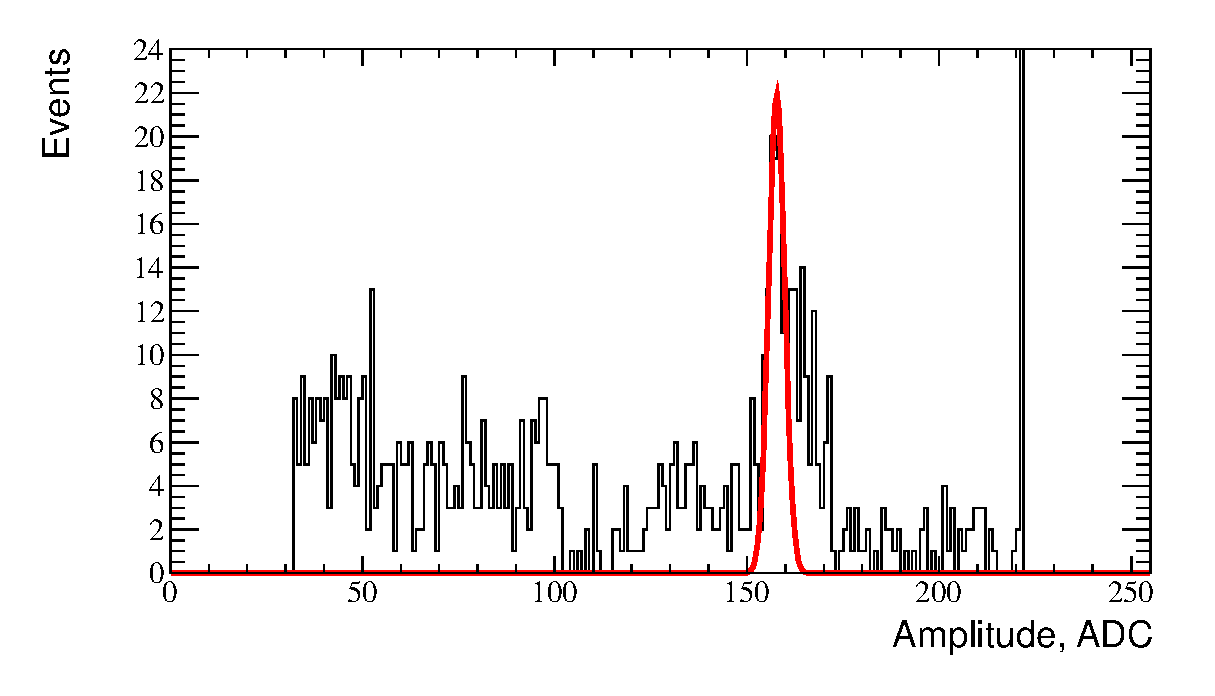
\includegraphics[width=\textwidth]{gfx/atten_1_over_3_ch06.eps}
\caption{Signal attenuated to $1/3$}
\end{subfigure}
\caption{Alpha peaks as seen with different on-board attenuator settings (Y2U).}
\label{fig:atten_distrib}
\end{figure}


\section{Conclusions}

Based on the analysis presented in this note we establish that the changes in
the bias currents in our silicon detectors heavily depend on the beam activity
in RHIC. At the moment, we do not see that the bias current correlates with
the beam intensity (\cref{fig:bc_vs_beamcurrent}) but in further studies we
plan to investigate if other beam or machine parameters have direct impact on
the detectors.

We observe a strong correlation between the gain and the bias current.
This variation goes as high as $\approx 20-40\%$ on the operational bias current
span (\cref{fig:bc_vs_gain}). We believe that the entire analysis
may benefit from a correction addressing such time-dependant fluctuations.
However, implementing it at the moment is not feasible due to
the fact that the bias current measurements are taken only once each five minutes.
This is enough to determine the average bias current for 20-minute long alpha runs, but
a regular sweep polarization measurement takes only a few seconds. It is not
unusual for the bias current to change significantly simultaneously with the sweep measurement (\cref{fig:bc_jumping}).
We believe that it would be better to have more frequent bias current measurements in the future.

The presence of the two $\alpha$-sources in the polarimeters allowed us to find
a correction for the effective detector gain by taking into account dead layer
energy losses. We find this correction (\cref{fig:gain_relations}) to be at $\approx 5\%$ level
with respect to the nominal calibration procedure with one radioactive source.
In addition, we estimate the thickness of the effective dead layer to be
$\approx 80\text{ }\mu g/cm^2$. This number disagrees with the value extracted
from the nominal ``banana'' fit to the carbon data where the effective dead layer is
estimated to be $\approx 35\text{ }\mu g/cm^2$ and the value of $1500\text{ }\angstrom$
($\approx 35\text{ }\mu g/cm^2$) provided by instrumentation group.
A possible explanation for this discrepancy
is that we overestimate the effective dead layer thickness as measured with
$\alpha$-particles by not taking into account the extra material of the protective
coating of the alpha source.

Comparing the detector gains measured before and after the beam time we conclude
that there was no significant radiation damage of the detectors.

A similar study has been performed for the 2012 data. The corresponding plots
can be found in \cref{sec:appendix_run12}.


\clearpage
\appendix
\section{Appendix: Run12 plots}
\label{sec:appendix_run12}

\begin{figure}[htb]
\begin{subfigure}[t]{0.49\textwidth}
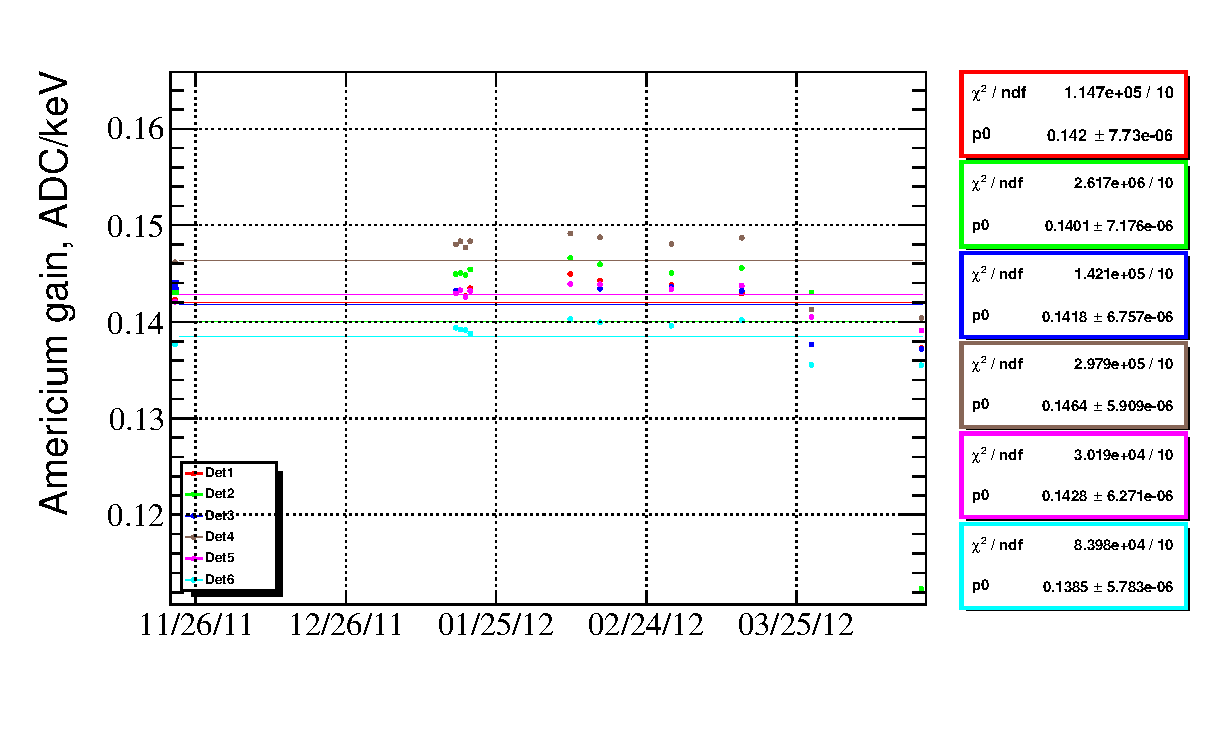
\includegraphics[width=\textwidth]{gfx/run12_alpha/B1U/c_chAmGain_by_day_B1U.eps}
\caption{B1U}
\end{subfigure}
%
\hfill
%
\begin{subfigure}[t]{0.49\textwidth}
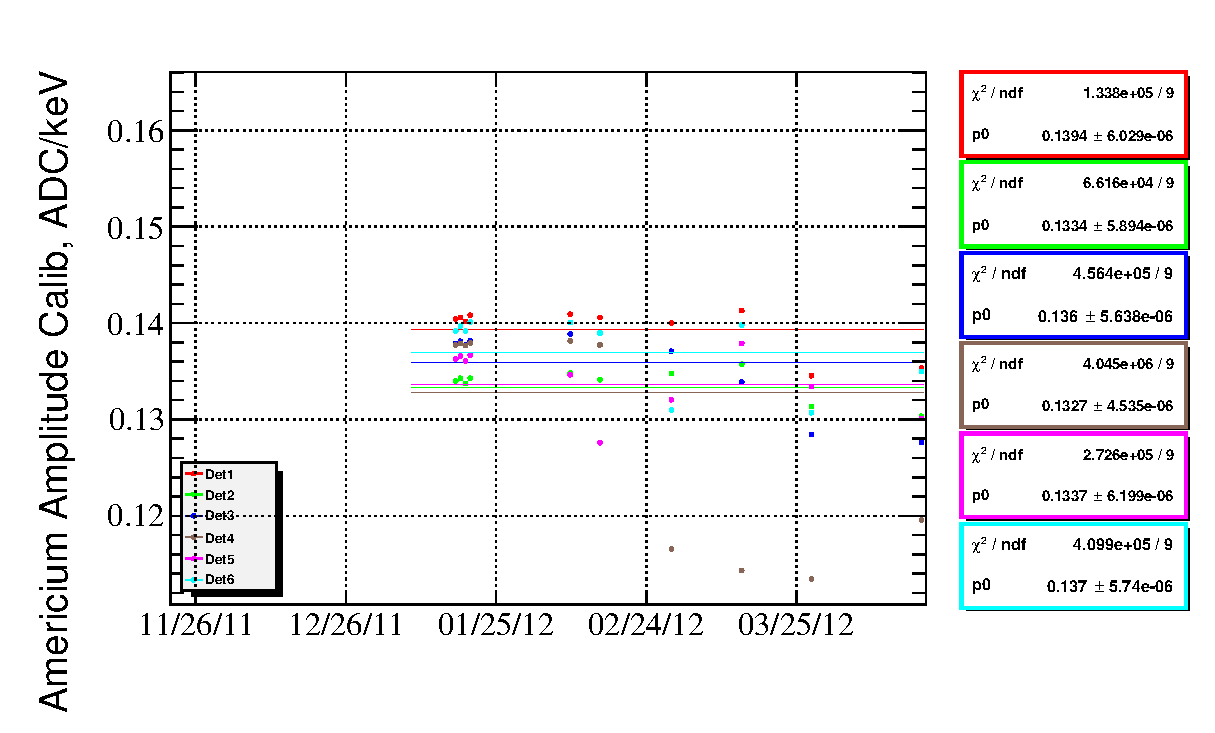
\includegraphics[width=\textwidth]{gfx/run12_alpha/Y1D/c_chAmGain_by_day_Y1D.eps}
\caption{Y1D}
\end{subfigure}

\begin{subfigure}[t]{0.49\textwidth}
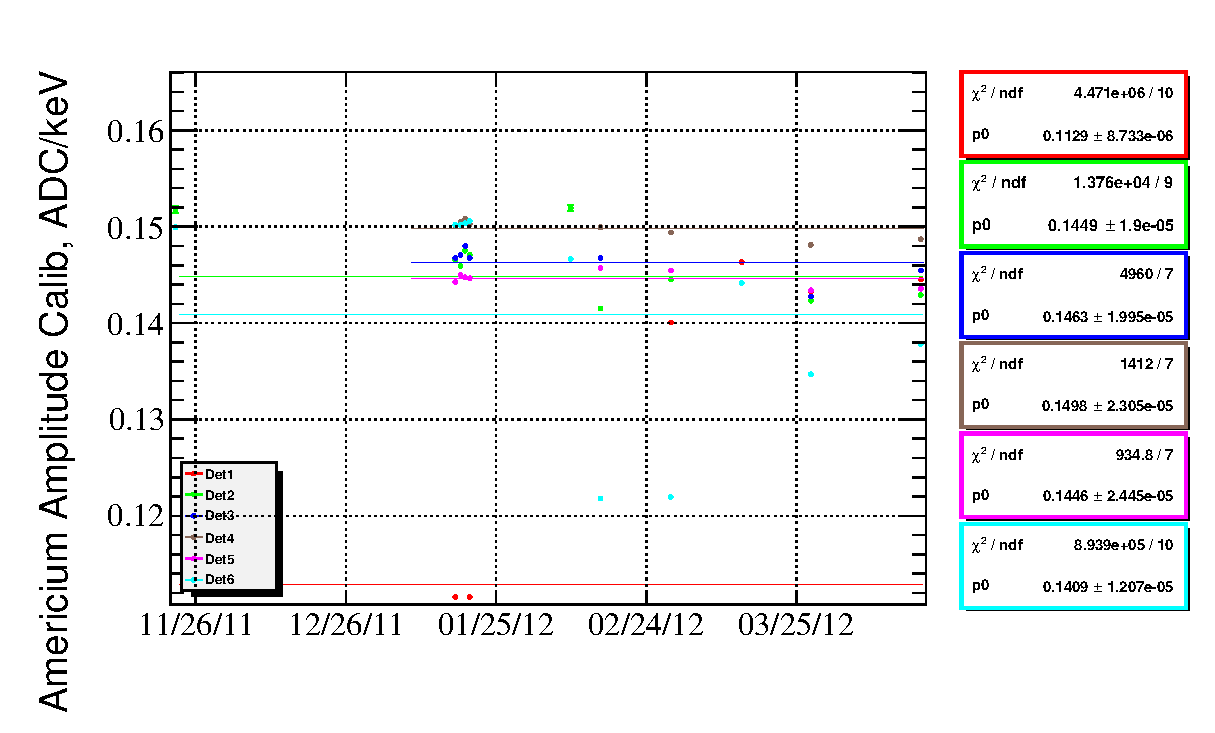
\includegraphics[width=\textwidth]{gfx/run12_alpha/B2D/c_chAmGain_by_day_B2D.eps}
\caption{B2D}
\end{subfigure}
%
\hfill
%
\begin{subfigure}[t]{0.49\textwidth}
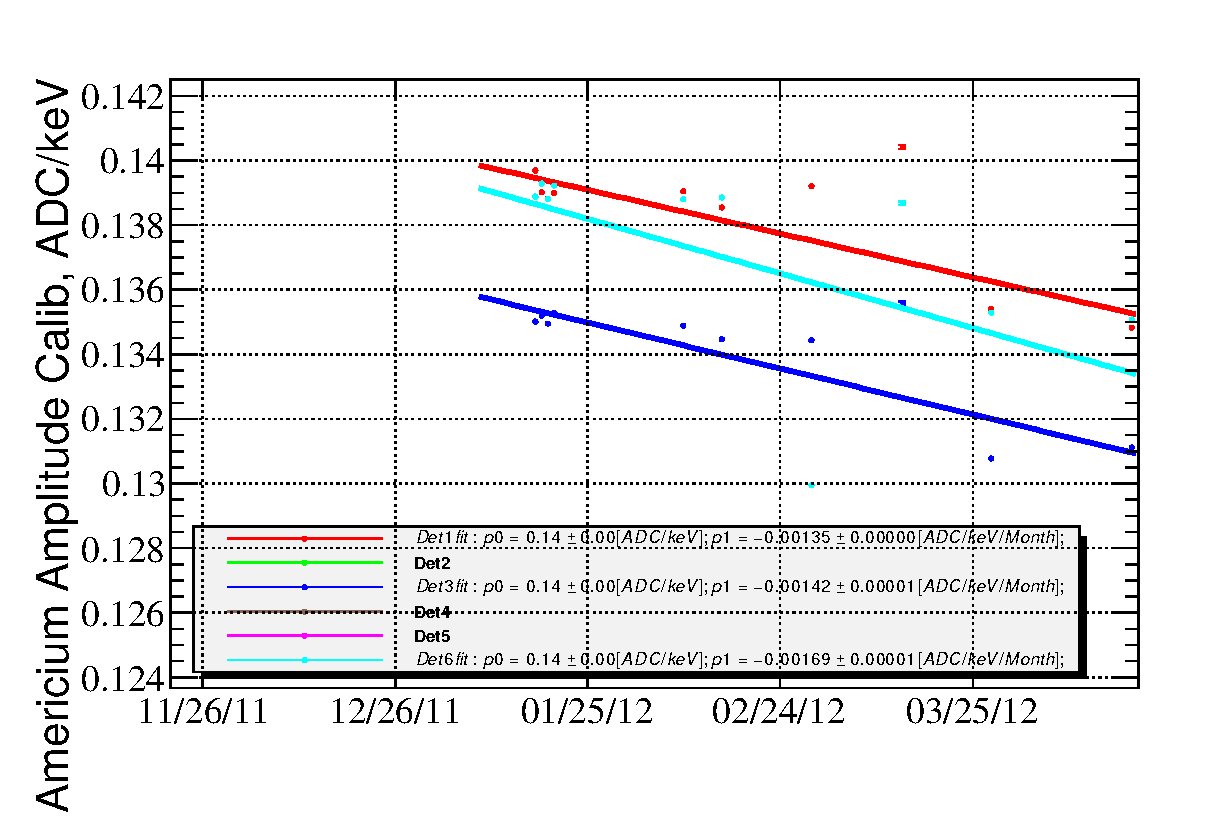
\includegraphics[width=\textwidth]{gfx/run12_alpha/Y2U/c_chAmGain_by_day_Y2U.eps}
\caption{Y2U}
\end{subfigure}
%
\caption{\amgainlabel{} (run12\_alpha)}
\end{figure}

\begin{figure}[htb]
\begin{subfigure}[t]{0.49\textwidth}
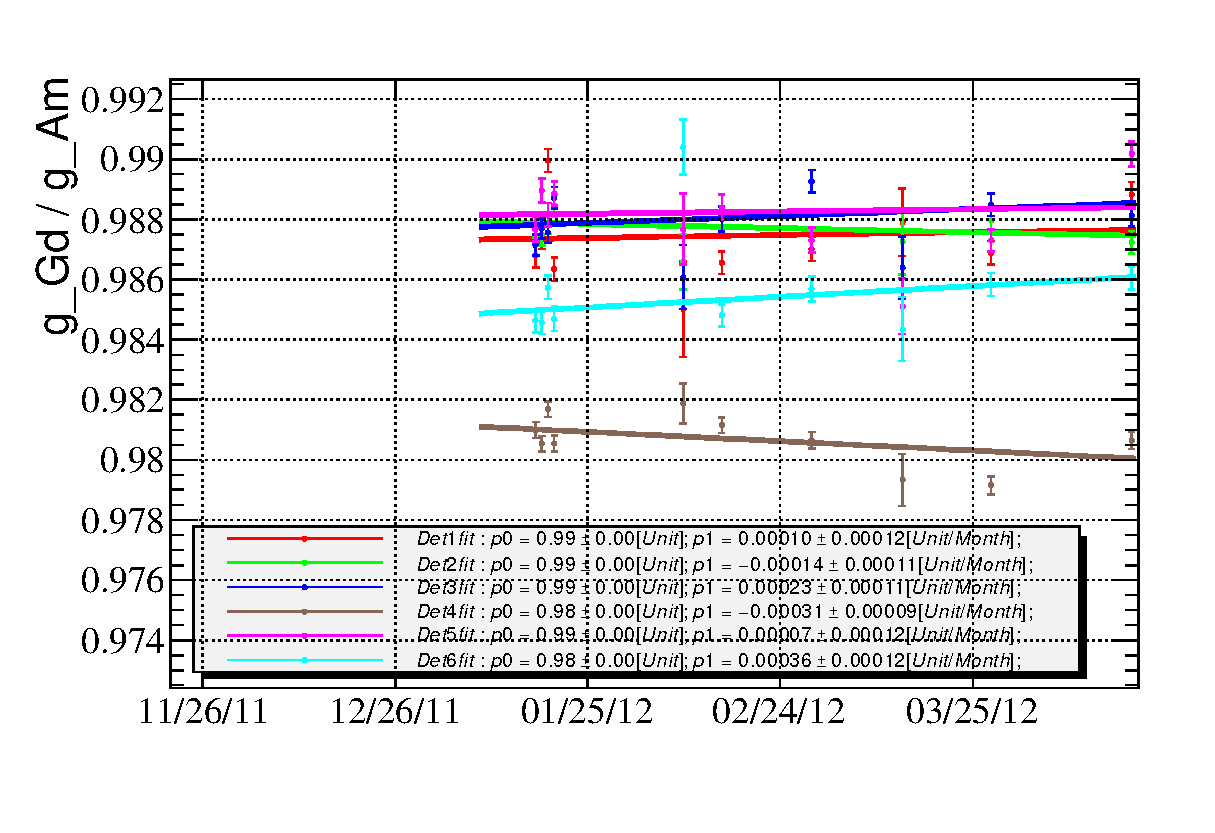
\includegraphics[width=\textwidth]{gfx/run12_alpha/Y2U/c_chGdGain_over_AmGain_by_day_Y2U.eps}
\caption{Relation of gadolinium and americium gains for \textbf{Y2U} polarimeter.}
\end{subfigure}
%
\hfill
%
\begin{subfigure}[t]{0.49\textwidth}
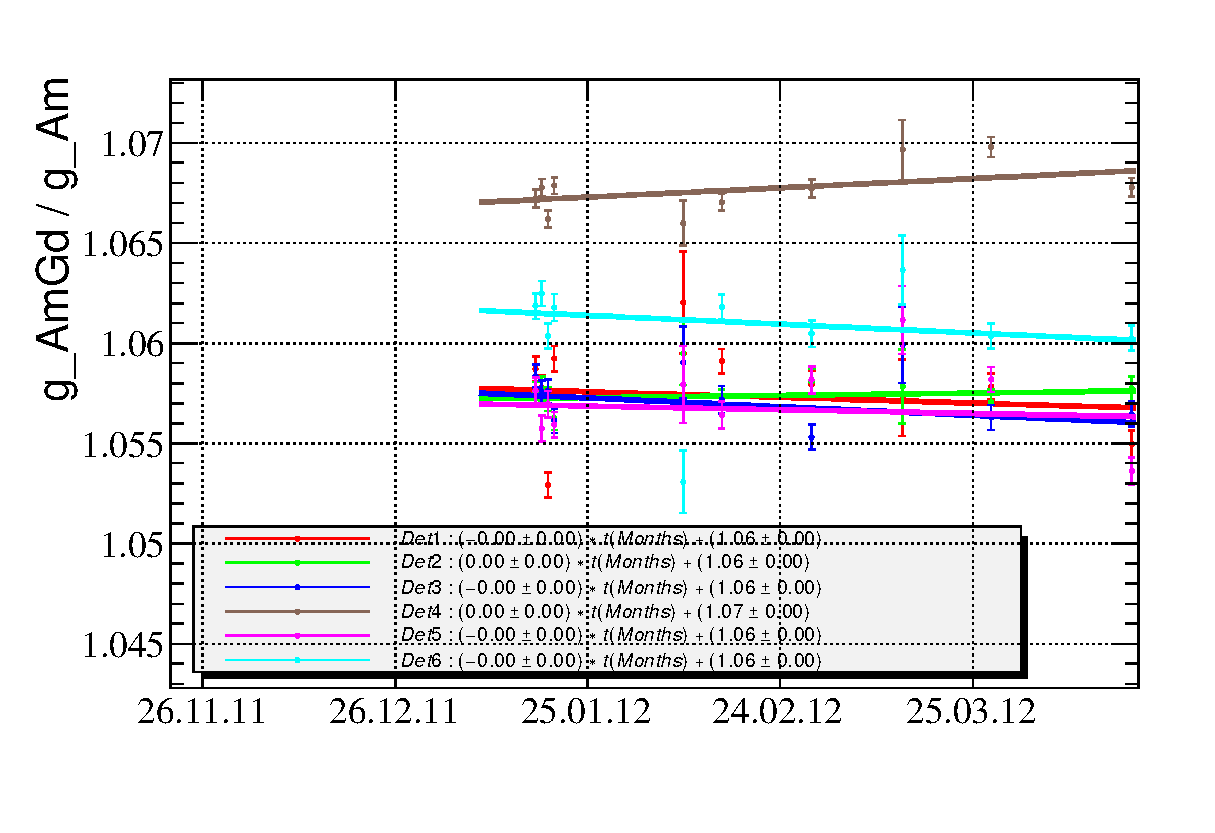
\includegraphics[width=\textwidth]{gfx/run12_alpha/Y2U/c_chAmGdGain_over_AmGain_by_day_Y2U.eps}
\caption{Relation of two-point (americium and gadolinium) linear fit slope and americium gain
for \textbf{Y2U} polarimeter.}
\end{subfigure}
%
\begin{subfigure}[t]{0.49\textwidth}
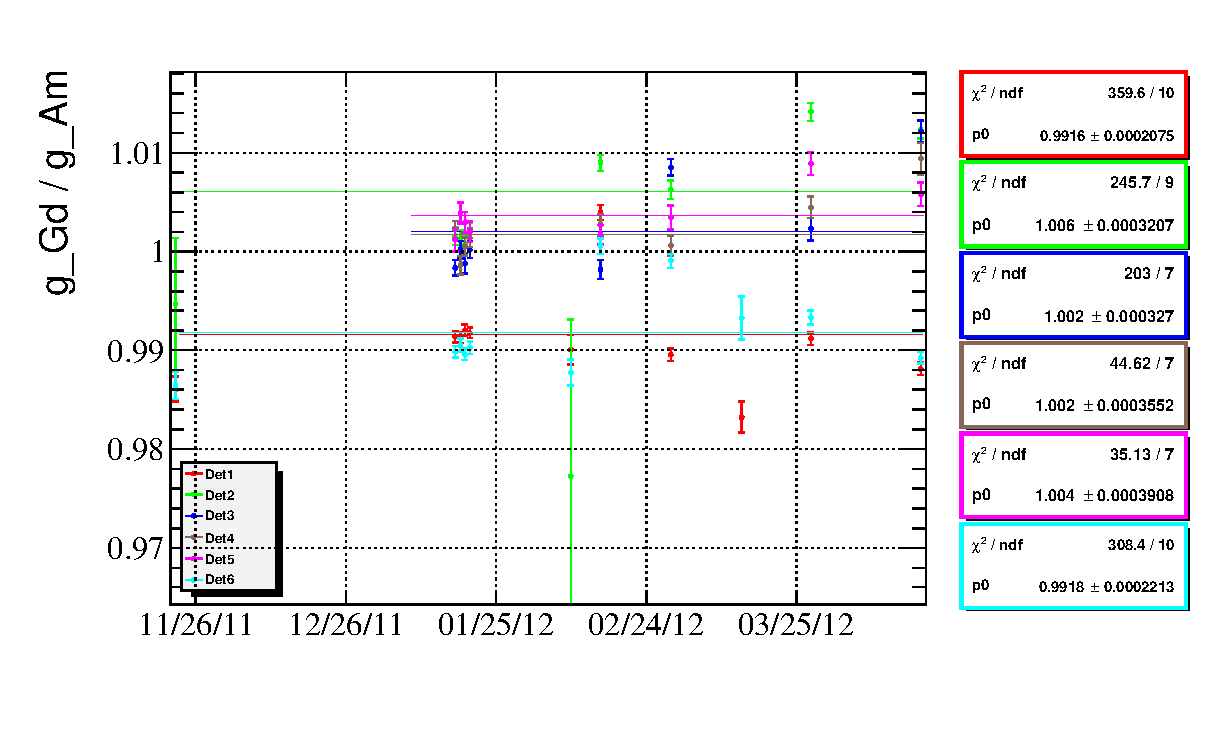
\includegraphics[width=\textwidth]{gfx/run12_alpha/B2D/c_chGdGain_over_AmGain_by_day_B2D.eps}
\caption{Relation of gadolinium and americium gains for \textbf{B2D} polarimeter.}
\end{subfigure}
%
\hfill
%
\begin{subfigure}[t]{0.49\textwidth}
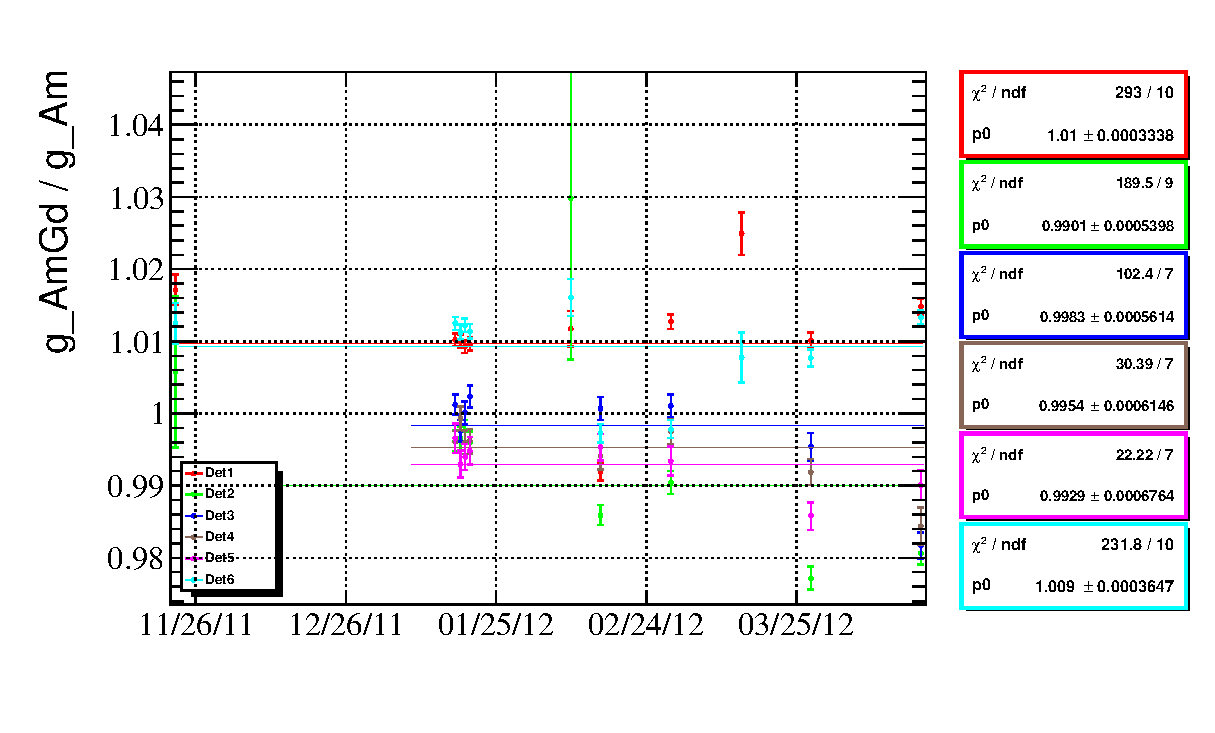
\includegraphics[width=\textwidth]{gfx/run12_alpha/B2D/c_chAmGdGain_over_AmGain_by_day_B2D.eps}
\caption{Relation of two-point (americium and gadolinium) linear fit slope and americium gain
for \textbf{B2D} polarimeter.}
\end{subfigure}
\caption{\gainrealationslabel{} (run12\_alpha)}
\end{figure}

\begin{figure}[htb]
\begin{subfigure}[t]{0.49\textwidth}
\includegraphics[width=\textwidth]{gfx/run12_alpha/B2D/c_chDeadLayerEnergy_by_day_B2D.eps}
\caption{B2D}
\end{subfigure}
%
\hfill
%
\begin{subfigure}[t]{0.49\textwidth}
\includegraphics[width=\textwidth]{gfx/run12_alpha/Y2U/c_chDeadLayerEnergy_by_day_Y2U.eps}
\caption{Y2U}
\end{subfigure}
\caption{\edllabellabel{} (run12\_alpha)}
\end{figure}

\begin{figure}[htb]
\begin{subfigure}[t]{0.49\textwidth}
\includegraphics[width=\textwidth]{gfx/run12_alpha/B2D/c_chDeadLayerSize_by_day_B2D.eps}
\caption{B2D}
\end{subfigure}
%
\hfill
%
\begin{subfigure}[t]{0.49\textwidth}
\includegraphics[width=\textwidth]{gfx/run12_alpha/Y2U/c_chDeadLayerSize_by_day_Y2U.eps}
\caption{Y2U}
\end{subfigure}
\caption{\xdllabel{} (run12\_alpha)}
\end{figure}

\begin{figure}[htb]
\begin{subfigure}[t]{0.49\textwidth}
\includegraphics[width=\textwidth]{gfx/run12_alpha/B2D/c_hBiasCurrent_DeadLayerSize.eps}
\caption{B2D}
\end{subfigure}
%
\hfill
%
\begin{subfigure}[t]{0.49\textwidth}
\includegraphics[width=\textwidth]{gfx/run12_alpha/Y2U/c_hBiasCurrent_DeadLayerSize.eps}
\caption{Y2U}
\end{subfigure}
\caption{\bcvsxdllabel{} (run12\_alpha)}
\end{figure}

\begin{figure}[htb]
\begin{subfigure}[t]{0.49\textwidth}
\includegraphics[width=\textwidth]{gfx/run12_alpha/B1U/c_hBiasCurrent_AmGain.eps}
\caption{B1U}
\end{subfigure}
%
\hfill
%
\begin{subfigure}[t]{0.49\textwidth}
\includegraphics[width=\textwidth]{gfx/run12_alpha/Y1D/c_hBiasCurrent_AmGain.eps}
\caption{Y1D}
\end{subfigure}

\begin{subfigure}[t]{0.49\textwidth}
\includegraphics[width=\textwidth]{gfx/run12_alpha/B2D/c_hBiasCurrent_AmGain.eps}
\caption{B2D}
\end{subfigure}
%
\hfill
%
\begin{subfigure}[t]{0.49\textwidth}
\includegraphics[width=\textwidth]{gfx/run12_alpha/Y2U/c_hBiasCurrent_AmGain.eps}
\caption{Y2U}
\end{subfigure}
%
\caption{\bcvsgainlabel{} (run12\_alpha)}
\end{figure}


\clearpage
\begin{thebibliography}{9} % for less than 10 references use just {9}

\bibitem{cnipol_code}
RHIC polarimetry analysis framework: \url{https://github.com/rhicspin/cnipol}

\bibitem{rytz}
A. Rytz, \emph{At. Data and Nucl. Data Tables} \textbf{47}, 205 (1991).

\bibitem{astar_database}
ASTAR database. Stopping power and range tables for helium atoms:
\url{http://physics.nist.gov/PhysRefData/Star/Text/ASTAR.html}

\bibitem{schmidke_edep}
B. Schmidke,
\emph{Carbon \& alpha E-deposition in Si}, July 8 (special meeting)
\url{https://wiki.bnl.gov/rhicspin/upload/7/72/Schmidke_Special_meeting_08.07.13.pdf}

\bibitem{schmidke_alpha_vs_carbon}
B. Schmidke,
\emph{Alpha gain <-> carbon gain}, August 16 (special meeting)
\url{https://wiki.bnl.gov/rhicspin/upload/f/fe/Schmidke_Special_meeting_16.08.13.pdf}

\bibitem{dkalinkin_bc_vs_carbongain}
D. Kalinkin,
\emph{Carbon gain vs. Ibias} (see slide 7), August 16 (special meeting)
\url{https://wiki.bnl.gov/rhicspin/upload/5/5f/Dkalinkin_16-08-13.pdf}

\bibitem{cnipol_web_rundb}
RHIC polarimetry results: \url{http://www.phy.bnl.gov/cnipol/rundb/}

\end{thebibliography}

\end{document}
